%%%%%%%%%%%%%%%%%%%%%%%%%%%%%%%%%%%%%%%%%%%%%%%%%%%%%%%%%%
%
% Doctoral Thesis Template @ The University of Manchester
% LaTeX Chapter Template
% Version 1 (23/07/2020)
% Joe Crone
%
% This template is based on:
% The University of Manchester, Presentation of Thesis Policy
% Research Office Graduate Education Team
% June 2017
% http://www.regulations.manchester.ac.uk/pgr-presentation-theses/
%
%%%%%%%%%%%%%%%%%%%%%%%%%%%%%%%%%%%%%%%%%%%%%%%%%%%%%%%%%%
\documentclass[../main.tex]{subfiles}
\begin{document}

% Title
%--------------------------------------------------------
\chapter{Introduction}
\label{Introduction} % to reference use \ref{ChapterTemplate}

Energy Recovery Linacs (ERLs) are ideal drivers of inverse Compton scattering (ICS) photon sources due to the combination of linac quality beams and high repetition rate, allowing production of a tunable high-flux, narrowband scattered photon beam. Energy recovery linacs, specifically multi-turn ERLs, can accelerate electron beams on the 10's~\si{\mega\electronvolt}-scale to the \si{\giga\electronvolt}-scale within a small accelerator footprint whilst maintaining small normalised emittances on the order of 1~\si{\milli\meter}--\si{\milli\radian} and short bunches in the picosecond domain. Parameters such as these have been demonstrated by the first multi-turn superconducting ERL demonstration (at a lower electron beam current) with the 4-turn energy recovery commissioning run at the Cornell University Brookhaven National Laboratory Energy Recovery Linac Test Accelerator (CBETA) \cite{hoffstaetter2017cbeta,bartnik2020cbeta}. These are ideal parameters for accelerator production of radiation, especially radiation production from inverse Compton scattering because a high electron beam energy is required to generate short wavelength radiation and a small physical size of the interacted electron beam is required to generate a small, intense and monochromatic radiation beam. Exploitation of ERLs for radiation production has been demonstrated most prominently by the high average power Jefferson Laboratory Free Electron Laser (FEL) \cite{neil2006jlab}; both the ALICE \cite{priebe2010first} and cERL \cite{akagi2016narrow} single turn ERLs have previously demonstrated ERL based x-ray production from inverse Compton scattering, albeit at low flux as a consequence of their lower average electron beam current. 

Due to a $E_{\gamma} = 4\gamma^{2}E_{L}$ scattered photon energy $E_{\gamma}$ dependence (see Section~\ref{sec:intro_ICS}), where $\gamma$ is the Lorentz factor and $E_{L}$ the energy of the incident photon, ICS interactions are the prime candidate for production of high energy photons above the photon energies available at conventional x-ray production facilities such as FELs ($E_{\gamma} <$~25~keV \cite{schneidmiller2011photon}) and the largest synchrotrons ($E_{\gamma} <$~500~keV \cite{spring8beamlines}). Therefore, inverse Compton scattering sources are the eminent method for high-flux production of $\gamma$-rays ($E_{\gamma}>$~1~MeV). Application of high flux, monochromatic $\gamma$-ray sources to nuclear physics experiments would support applications like nuclear resonance fluorescence (NRF) \cite{hayakawa2010nondestructive} and nuclear photonics \cite{budker2021expanding}. The efficacy of $\gamma$-ray production by inverse Compton scattering for experimentation in nuclear physics has been proven by the HI$\gamma$S ICS source \cite{weller2009research} however, improvements in bandwidth (energy spread or linewidth of the produced radiation) are required for high resolution experiments. Hence, the flagship Extreme Light Infrastructure -- Nuclear Physics -- Gamma Beam System (ELI-NP-GBS) project \cite{adriani2014technical,elinp2019vega,tanaka2020current} has been designed for ICS production of $\gamma$-rays up to energies of 19.5~\si{\mega\electronvolt} in a narrow 0.5\% FWHM bandwidth \cite{elinp2019vega}. Whilst other $\gamma$-ray sources exist -- such as bremsstrahlung sources -- the ICS process offers unparalleled narrowband radiation production most favoured by experimentalists because ICS sources can be optimised to produce photons in a smaller natural bandwidth than synchrotron radiation via simple collimation, alleviating the need for monochromation which inherently depletes the number of generated photons. However, collimation of 10's~\si{\mega\electronvolt} $\gamma$-rays becomes difficult because these can penetrate a large thickness of typical collimation materials such as lead.  

The current status of energy recovery linac development and the most common accelerator driven radiation production methods are now explained to provide the motivation for the development of ERL driven ICS sources. The review of ERLs focuses on radiation production, specifically the development of high energy and high average beam current ERLs which are key for short wavelength photon production ($\lambda \lesssim 1$~\si{\nano\meter}, $E_{\gamma} \gtrsim 1$~\si{\kilo\electronvolt}) and production of the maximum number of photons. Accelerator driven radiation production methods such as synchrotron radiation facilities, free electron lasers and bremsstrahlung sources are reviewed because these are the production methods most relevant to production of large quantities of short wavelength photons. The scope and structure of the thesis is then explained in Section~\ref{sec:thesis_layout_scope}.    

\section{Energy Recovery Linacs}

The energy recovery linac is a re-circulated linac concept invented by M. Tigner in 1965 \cite{tigner1965possible} to improve the power consumption of particle colliders by re-circulating the particle beam post-interaction for recovery of its kinetic energy in the same radio-frequency (RF) cavities that provided the initial acceleration. Diagrams of the ERL as envisaged by Tigner, and the now--common racetrack design, are shown in Fig.~\ref{fig:tigner_modern_ERL}. The recovered energy can then be applied to accelerate a following electron bunch, without additional application of RF power, thereby recycling the RF power of the particle accelerator. Another benefit is that the particle beam is decelerated during the energy recovery process therefore the kinetic energy and power of the dumped particle beam is reduced. A more detailed explanation of an energy recovery linac is presented in Chapter~\ref{Energy_Recovery_Linac_Design}.
\begin{figure}[!h]
\centering
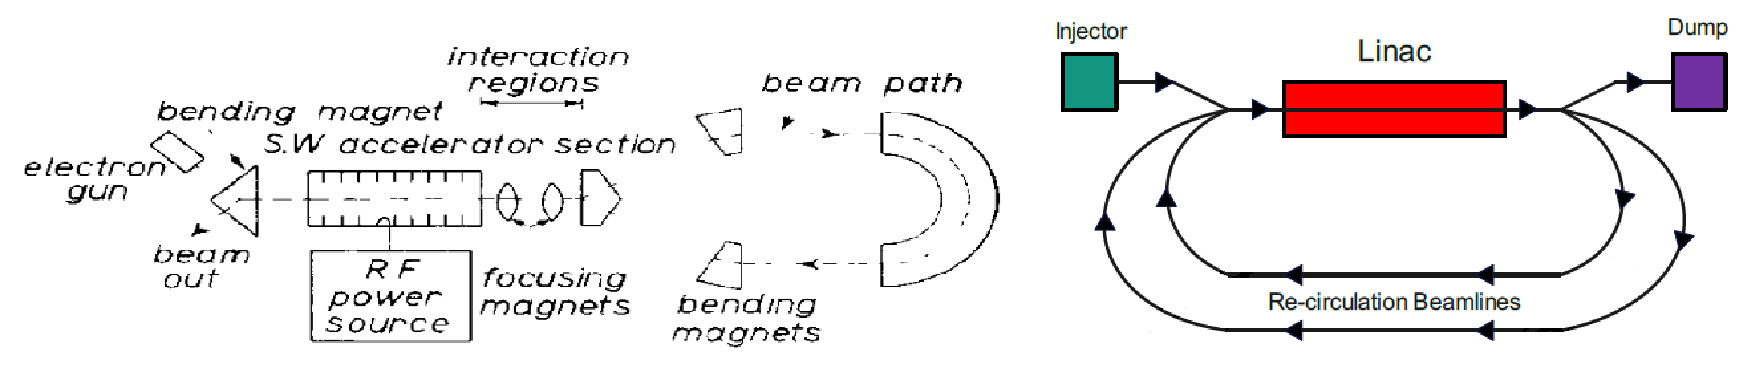
\includegraphics[width=\textwidth]{Figures/Introduction/Tigner_Modern_ERL.pdf}
\caption{Left: Originally envisioned ERL collider `clashing beam experiment' reproduced from Tigner \cite{tigner1965possible}. A  particle bunch produced from the electron gun is accelerated then re-circulated whilst another electron bunch is generated, the two electron beams collide and the initial electron bunch is decelerated and dumped. Right: A multi-turn ERL where an electron bunch is generated by the injector (electron gun) then accelerated by the linac, the electron beam is then re-circulated until it enters the linac where it is accelerated again. The electron beam is then re-circulated again for two passes of the linac and decelerated in each pass and then directed to the beam dump. This is the basic scheme of a multi-turn ERL.}
\label{fig:tigner_modern_ERL}
\end{figure}

The ERL concept was first demonstrated in the superconducting accelerator driven Free Electron Laser (SCA/FEL) \cite{smith1987development} -- the first superconducting RF (SRF) ERL. SCA/FEL was capable of producing $E_{e} = 93$~\si{\mega\electronvolt} electron bunches with 5~\si{\milli\meter}--\si{\milli\radian} normalised emittance, a 5~\si{\pico\second} bunch duration and 150~\si{\micro\ampere} average beam current. SCA/FEL contained a single electron bunch which was re-circulated around the ERL before the next bunch was produced. As well as being the first demonstration of an ERL, the SCA/FEL demonstrated the efficacy of an ERL as a driver of a light source by demonstrating a UV FEL operating at $\lambda = 200$~\si{\nano\meter}. Unlike Tigner's initial vision of ERLs as particle colliders \cite{tigner1965possible}, ERL particle beams have consistently been applied to drive radiation production.

ERLs have also been demonstrated using normal conducting RF (NCRF) cavities, such as the Chalk River Reflexotron ($E_{e} = 25$~\si{\mega\electronvolt}) \cite{schriber1977experimental} and the Los Alamos FEL ($E_{e} = 23.5$~\si{\mega\electronvolt})\cite{feldman1987energy}, however these are typically low electron energy machines ($E_{e} < 30$~\si{\mega\electronvolt}). Normal conducting ERLs are limited because NCRF accelerating cavities are susceptible to cavity losses and RF transport losses \cite{adolphsen2022european} in comparison to SRF cavities, therefore the increase in efficiency -- re-use of RF power -- from energy recovery is less beneficial because the RF power is dissipated. Superconducting RF cavities are typically far more power efficient than normal conducting accelerators; for example, the NC RF cavities used in the LEP accelerator have an efficiency of 15\% whereas the SRF cavities in LEP have an efficiency of 75\% \cite{weingarten1996superconducting}. As more RF cavities are required for acceleration of particles to higher energies the power dissipation problems in NCRF is exacerbated by ERL based production of short wavelength radiation, which requires higher energy particle beams. For high average beam current (10's~\si{\milli\ampere}) and beyond moderate energies ($E_{e} > 100$~\si{\mega\electronvolt}) with efficient use of RF acceleration, the development of superconducting RF ERLs is required. Consequently, high average electron beam powers are also readily available from SRF ERLs; for example, the ERL in the proposed 4GLS project \cite{poole20034gls} was predicted to have an electron beam power of 55~\si{\mega\watt} for a 550~\si{\mega\electronvolt} electron beam with a 100~\si{\milli\ampere} average beam current \cite{williams2007electron}. Hence, superconducting ERLs are the chosen technology for radiation production because the quantity of photons generated is increased with increasing average beam current. 

The demonstrated ERLs discussed so far were demonstrated using pulsed trains of electron bunches; however, continuous wave (CW) ERLs with continually produced electron bunches (see Section~\ref{sec:high_current_ERL}) can improve the average beam current of ERLs. Continuous wave ERLs were first demonstrated \cite{neil2000sustained} by the IR FEL demo \cite{benson1999first,neil2000sustained} at Jefferson Laboratory (JLab), where a single turn ERL was used to drive an infrared (IR) FEL. The JLab IR FEL demo, as shown in Fig.~\ref{fig:J_Lab_FEL_diagram}, produced an average beam current of 4.8~\si{\milli\ampere} with a 48~\si{\mega\electronvolt} electron energy for production of $\lambda =$ 3--5.3~\si{\micro\meter} infrared radiation with an average power of 1.72~\si{\kilo\watt}. Subsequently, with experience operating the IR FEL demo, an upgraded JLab IR FEL was designed \cite{benson2002have} and built \cite{behre2004first} with an upgraded higher average beam current injector, improved beam dynamics design and improved FEL design. The JLab IR FEL upgrade produced an average beam current of 9.1~\si{\milli\ampere} (the current record for SRF ERLs) with a 160~\si{\mega\electronvolt} electron energy -- a total beam power of 1.46~\si{\mega\watt} \cite{neil2006jlab}. The IR Upgrade ERL demonstrated this electron beam average power with only around 300~\si{\kilo\watt} of installed RF power \cite{adolphsen2022european}, which demonstrates the ability of the ERL concept to produce high power light sources whilst minimising the required electrical power. However, the power of the JLab FEL was primarily limited by the photoinjector gun \cite{hannon2008high}; a photoinjector capable of delivering a high average beam current is crucial to the development of high average beam current ERLs with many studies \cite{hannon2008high,dunham2013record,neumann2013towards} targeting 100~\si{\milli\ampere}.   
\begin{figure}[!h]
\centering
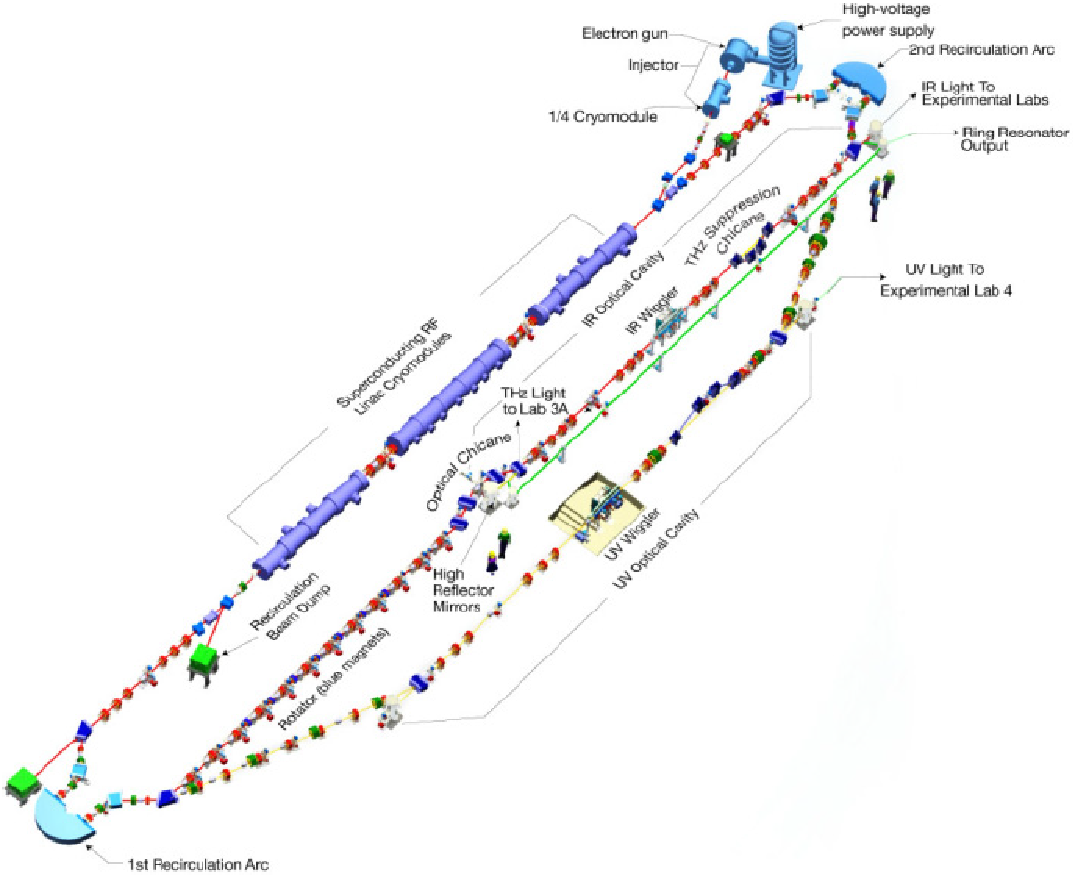
\includegraphics[width=0.7\textwidth]{Figures/Introduction/JLab_FEL.pdf}
\caption{Diagram of the JLab FEL upgrade. The JLab FEL is a single turn CW SRF ERL which drives a high average power ($P = 1.46$~\si{\mega\watt}) IR FEL. Currently, the JLab FEL has demonstrated the highest electron beam average current ($I_{\mathrm{avg}} = 9.1$~\si{\milli\ampere}) of any superconducting ERL. Reproduced from Benson et al \cite{benson2009jlamp}.}
\label{fig:J_Lab_FEL_diagram}
\end{figure}

The Continuous Electron Beam Accelerator Facility (CEBAF) \cite{bogacz2003cebaf,tennant2003beam} has subsequently demonstrated energy recovery at JLab, though CEBAF was originally designed as a re-circulated linac. A re-circulated linac differs from an energy recovery linac because a re-circulated linac accelerates the electron beam in multiple linac passes but does not then decelerate the electron beam; it is dumped at high energy. CEBAF demonstrated single turn energy recovery in 2003 \cite{bogacz2003cebaf,tennant2003beam} with energy recovery of a 1.02~\si{\giga\electronvolt} electron beam, the highest energy electron beam energy recovered, with a normalised transverse emittance of $\epsilon_{nx} \left(\epsilon_{ny}\right) = 2.39 \left(2.06\right)$~\si{\milli\meter}--\si{\milli\radian} \cite{tennant2003beam}. However, the average beam power of the CEBAF energy recovery demonstration was modest at 81.6~\si{\kilo\watt} because of the small average beam current $I_{\mathrm{avg}} = 80$~\si{\micro\ampere} \cite{freyberger2004cebaf}. Higher electron energies enable ERLs to be used for applications such as $\gamma$-ray production by ICS sources\cite{budker2021expanding} and in particle colliders such as the LHeC electron--hadron collider \cite{agostini2021large}, therefore higher energy ERL demonstrations like CEBAF are required.   

Since demonstration of the JLab FEL, larger ERL average beam currents have been pursued by the compact ERL (cERL) at KEK \cite{akagi2016narrow}, where demonstration of a 10~\si{\milli\ampere} average beam current is planned with near-100\% energy recovery efficiency \cite{adolphsen2022european}. A diagram of cERL is shown in Fig.~\ref{fig:cERL_ALICE_diagram}. Currently, an average beam current of 1~\si{\milli\ampere} has been achieved at cERL \cite{obina20191} with near-full energy recovery. Light sources other than FELs have been demonstrated at ERLs, such as the ICS source at the ALICE ERL (shown in Fig.~\ref{fig:cERL_ALICE_diagram}) at Daresbury Laboratory \cite{priebe2008inverse,priebe2010first}, the first SRF ERL in Europe primarily used as an ERL IR FEL \cite{thompson2014status}, and the ICS source applied to cERL \cite{akagi2016narrow}. ICS sources take advantage of the high electron beam brightness delivered by an ERL much like FELs. However, ICS source demonstrations upon ERLs have been limited to low energies (ALICE $E_{e}=30$~\si{\mega\electronvolt}, cERL  $E_{e}=20$~\si{\mega\electronvolt}) and low current $I < 1$~\si{\milli\ampere}, so only x-ray photons at low fluxes could be produced.
\begin{figure}[!h]
\centering
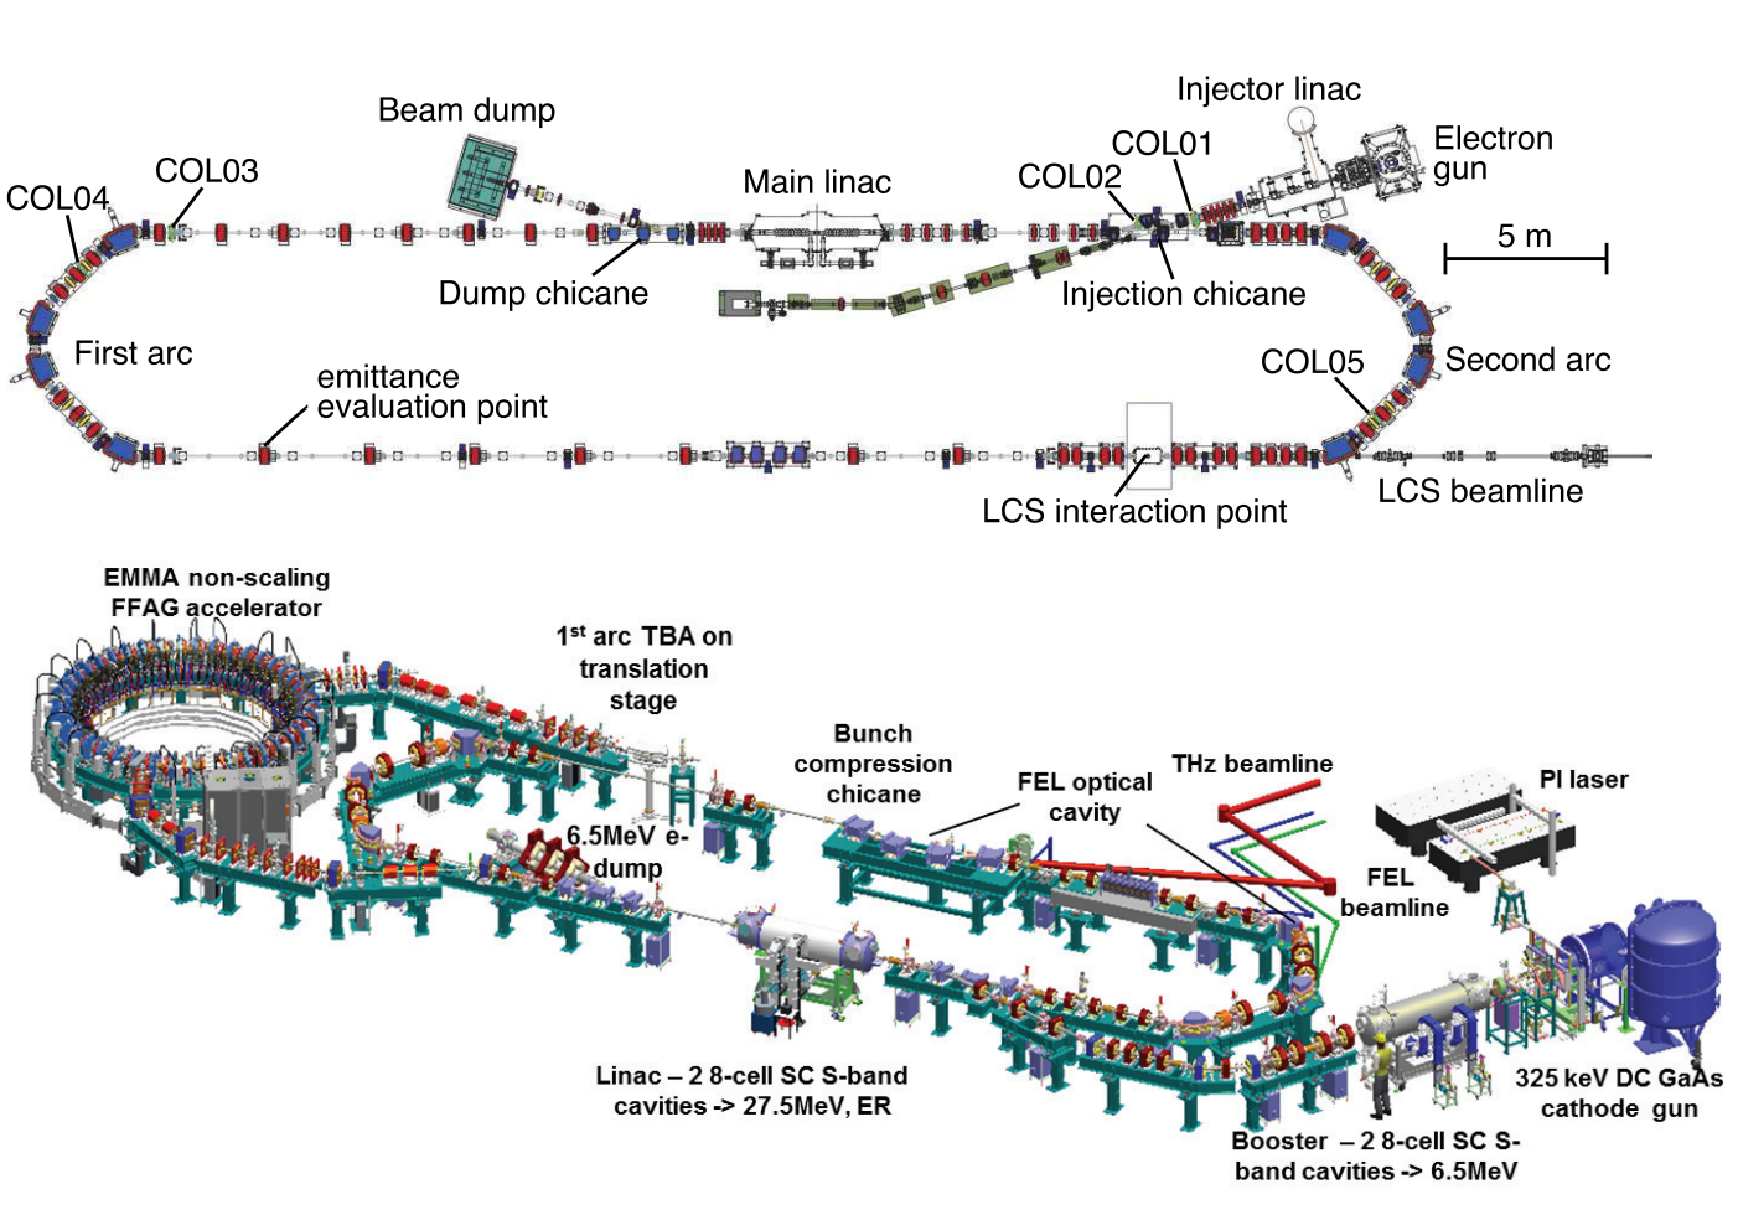
\includegraphics[width=0.8\textwidth]{Figures/Introduction/cERL_ALICE.pdf}
\caption{Top: The cERL single turn SRF ERL. cERL aims to demonstrate a 10~\si{\milli\ampere} average beam current, with 1~\si{\milli\ampere} previously demonstrated. cERL demonstrated the highest flux ICS source from an ERL. Reproduced from Akagi et al \cite{akagi2016narrow}. Bottom: The ALICE single turn ERL and EMMA non-scaling FFA. ALICE provided the first demonstration of an ICS source on an ERL -- COBALD. Reproduced from Thomson et al \cite{thompson2014status}.}
\label{fig:cERL_ALICE_diagram}
\end{figure}

The Novosibirsk Recuperator is a NCRF ERL that is used to drive terahertz photon production and three IR FELs. It is the first demonstrated multi-turn ERL \cite{gavrilov2007status}, where the electron bunch is accelerated for multiple passes before deceleration for multiple passes. Diagrams of a more simple multi-turn ERL and the Novosibirsk Recuperator are shown in Figs.~\ref{fig:tigner_modern_ERL} and \ref{fig:novosibirsk_recuperator} respectively. Multi-turn ERLs are advantageous because the electron beam can be repetitively accelerated in the same linac, allowing for a larger maximum electron energy for the same RF acceleration section as a single turn ERL. For example, single turn NCRF ERLs such as the Reflexotron have achieved an electron beam energy of 25~\si{\mega\electronvolt} \cite{schriber1977experimental}, whereas the Novosibirsk recuperator accelerates electrons up to energies of 42~\si{\mega\electronvolt} \cite{shevchenko2020novosibirsk}. The highest average electron beam current in an ERL demonstrated at 30~\si{\milli\ampere} has also been achieved in the Novosibirsk FEL \cite{gavrilov2007status}. A recent simulation study for the upgrade of the RF gun has predicted up to 100~\si{\milli\ampere} average beam current \cite{matveev2020simulation}, which could provide an average beam current in an NCRF ERL an order of magnitude larger than the 9.1~\si{\milli\ampere} \cite{neil2006jlab} demonstrated for SRF ERLs.  
\begin{figure}[!h]
\centering
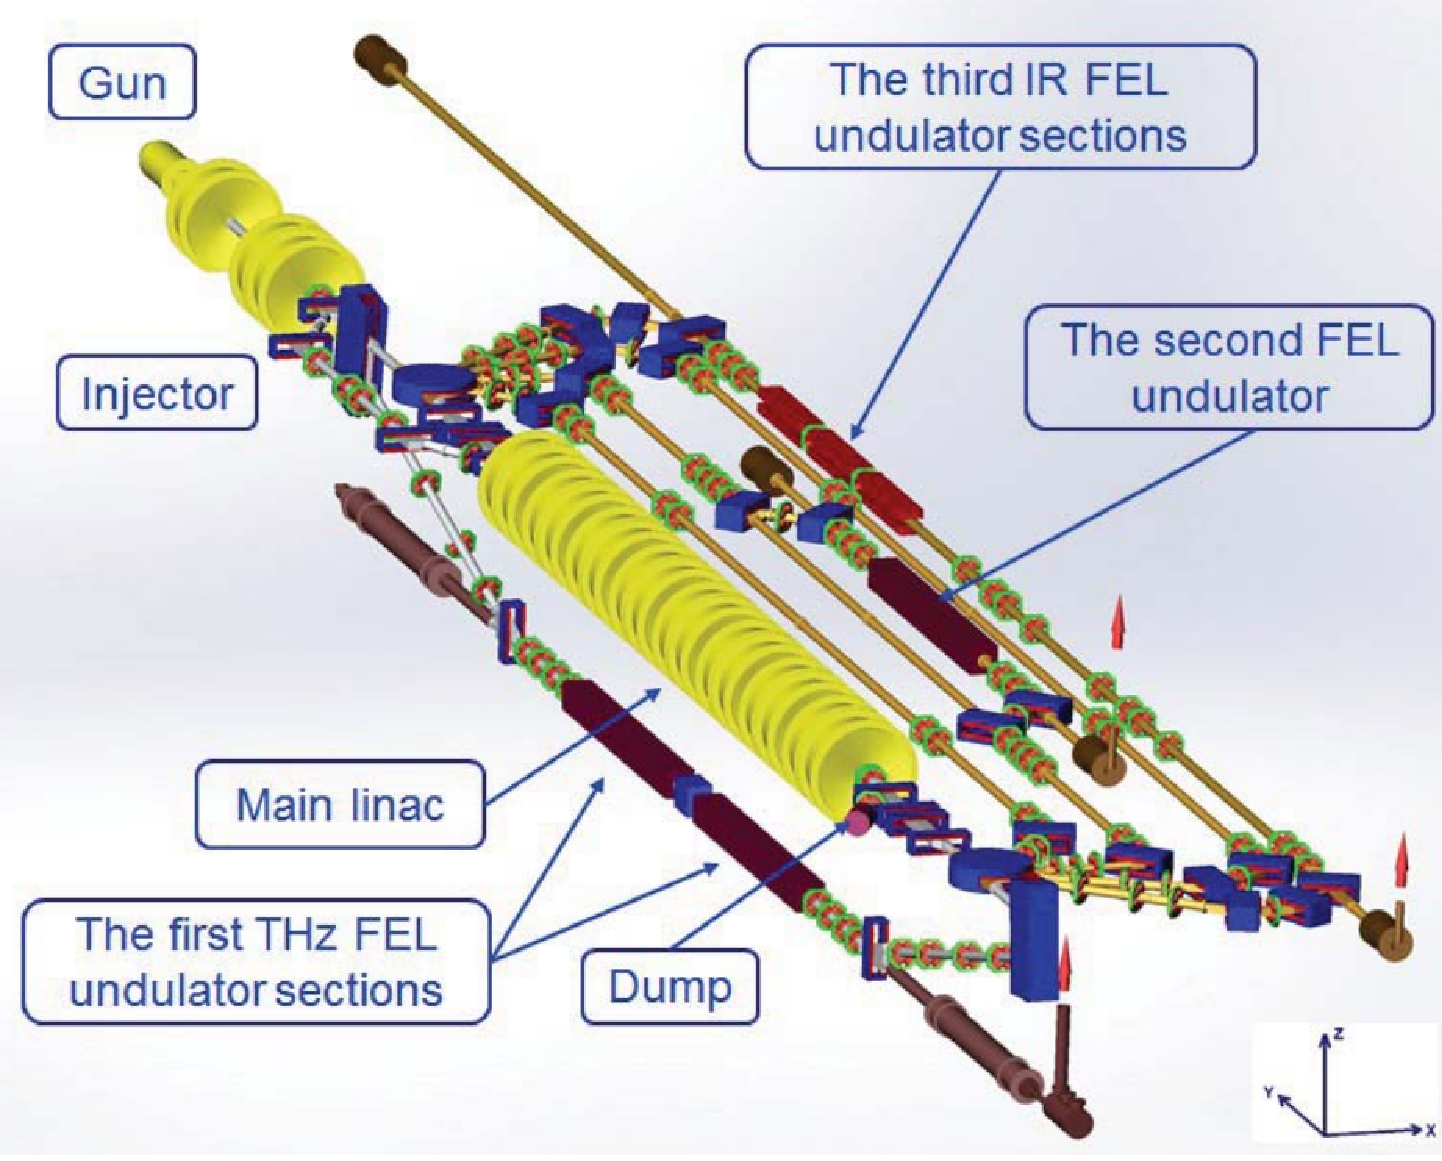
\includegraphics[width=0.6\textwidth]{Figures/Introduction/Novosibirsk_Recuperator.pdf}
\caption{The Novosibirsk Recuperator (NovoFEL) normal conducting 4-turn ERL. The electron beam from the Novosibirsk Recuperator drives a total of three FELs operating in the \si{\tera\hertz} ($\lambda = 90-340$~\si{\micro\meter}), far-infrared ($\lambda = 35 - 80$~\si{\micro\meter}) and near-infrared ($\lambda = 5 - 12$~\si{\micro\meter}) \cite{shevchenko2020novosibirsk} with an average beam current of up to 30~\si{\milli\ampere} \cite{gavrilov2007status}. Reproduced from Shevchenko et al \cite{shevchenko2020novosibirsk}. }
\label{fig:novosibirsk_recuperator}
\end{figure}

Multi-turn ERLs have been demonstrated with SRF accelerating structures firstly by the CBETA ERL \cite{bartnik2020cbeta} and then recently by S-DALINAC ERL \cite{arnold2020first,adolphsen2022european}; both are shown in Fig.~\ref{fig:CBETA_SDALINAC_diagram}. Up to 81.8\% of the electron bunch energy was recovered in S-DALINAC during multi-turn commissioning -- the highest energy recovery efficiency demonstrated for a multi-turn SRF ERL \cite{adolphsen2022european}. However, currently only low average beam currents have been demonstrated by multi-turn ERLs, with the S-DALINAC multi-turn ERL demonstrating maximum 8~\si{\micro\ampere} average beam current. The single turn CBETA ERL demonstrated a nominal electron beam energy of 42~\si{\mega\electronvolt} \cite{gulliford2021measurement}, whereas with the 4-turn configuration of CBETA a maximum electron beam energy of 150~\si{\mega\electronvolt} was demonstrated \cite{bartnik2020cbeta}; a factor of 3.57 increase in electron beam energy within a near-identical footprint to the single turn machine. CBETA commissioning is explained in more detail in Section~\ref{sec:CBETA_commissioning}, where a design of an ICS source driven by CBETA is proposed.
\begin{figure}[!h]
\centering
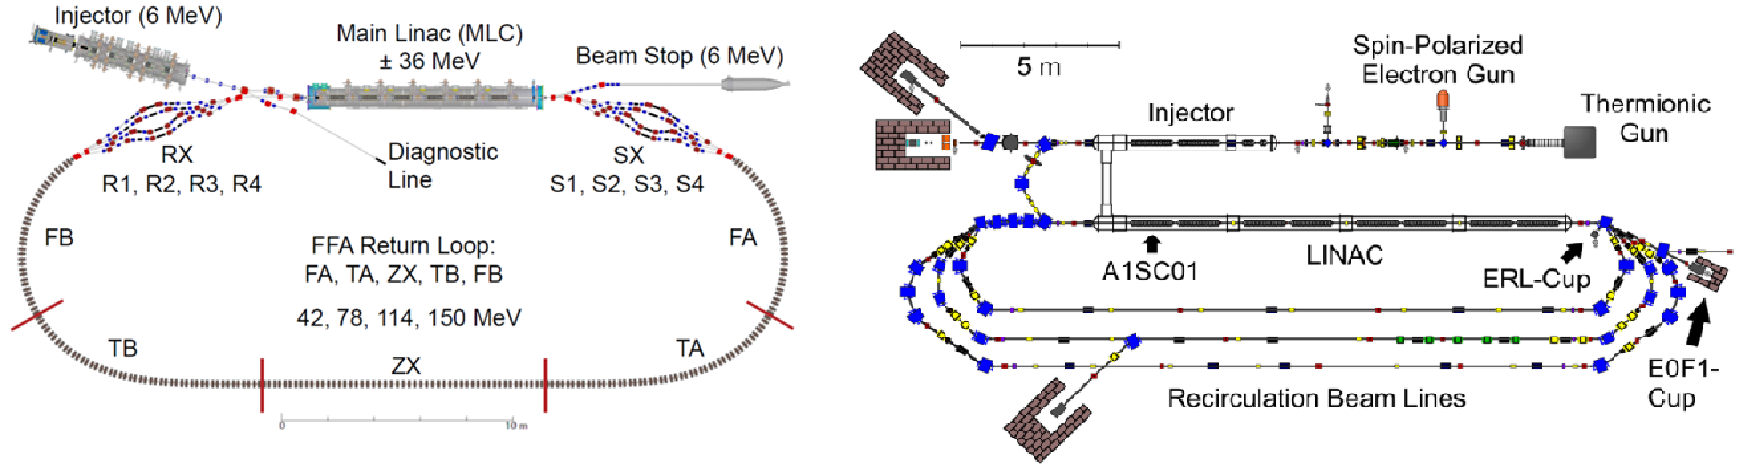
\includegraphics[width=\textwidth]{Figures/Introduction/CBETA_SDALINAC_diagram.pdf}
\caption{Left: The CBETA 4-turn SRF ERL designed to re-circulate electron beams with electron energies up to 150~\si{\milli\ampere} with a maximum electron beam average current of 40~\si{\milli\ampere} ($P = 6~\si{\mega\watt}$) \cite{hoffstaetter2017cbeta}. CBETA demonstrated 4-turn energy recovery with a small average beam current of 1~\si{\micro\ampere}. Right: The S-DALINAC 2-turn SRF ERL designed to re-circulate electron beams with energies up to 130~\si{\meg\electronvolt} and an average beam current of 20~\si{\milli\ampere} ($P = 2.6$~\si{\mega\watt}) \cite{arnold2017erl}. S-DALINAC demonstrated 2-turn energy recovery with a recovery efficiency of 81.8\% at an average beam current of 8~\si{\micro\ampere} \cite{adolphsen2022european}. Reproduced from Arnold et al \cite{arnold2020first}.}
\label{fig:CBETA_SDALINAC_diagram}
\end{figure}

A plot of the electron beam energy and beam current of various proposed and demonstrated ERL projects is shown in Fig.~\ref{fig:ERL_Landscape}. The maximum electron beam power demonstrated in an ERL is 1.46~\si{\mega\watt} using the JLab upgraded FEL \cite{neil2006jlab}, and the maximum electron beam energy demonstrated in an ERL is the $1.02$~\si{\giga\electronvolt} energy recovery demonstration using CEBAF \cite{bogacz2003cebaf,tennant2003beam}. However, several projects seek to demonstrate ERLs with higher average current, higher electron bunch energies and multi-turn designs, such as PERLE \cite{angal2018perle}, bERLinPro \cite{kuske2012conceptual} and ER@CEBAF \cite{meot2016er}.
\begin{figure}[!h]
\centering
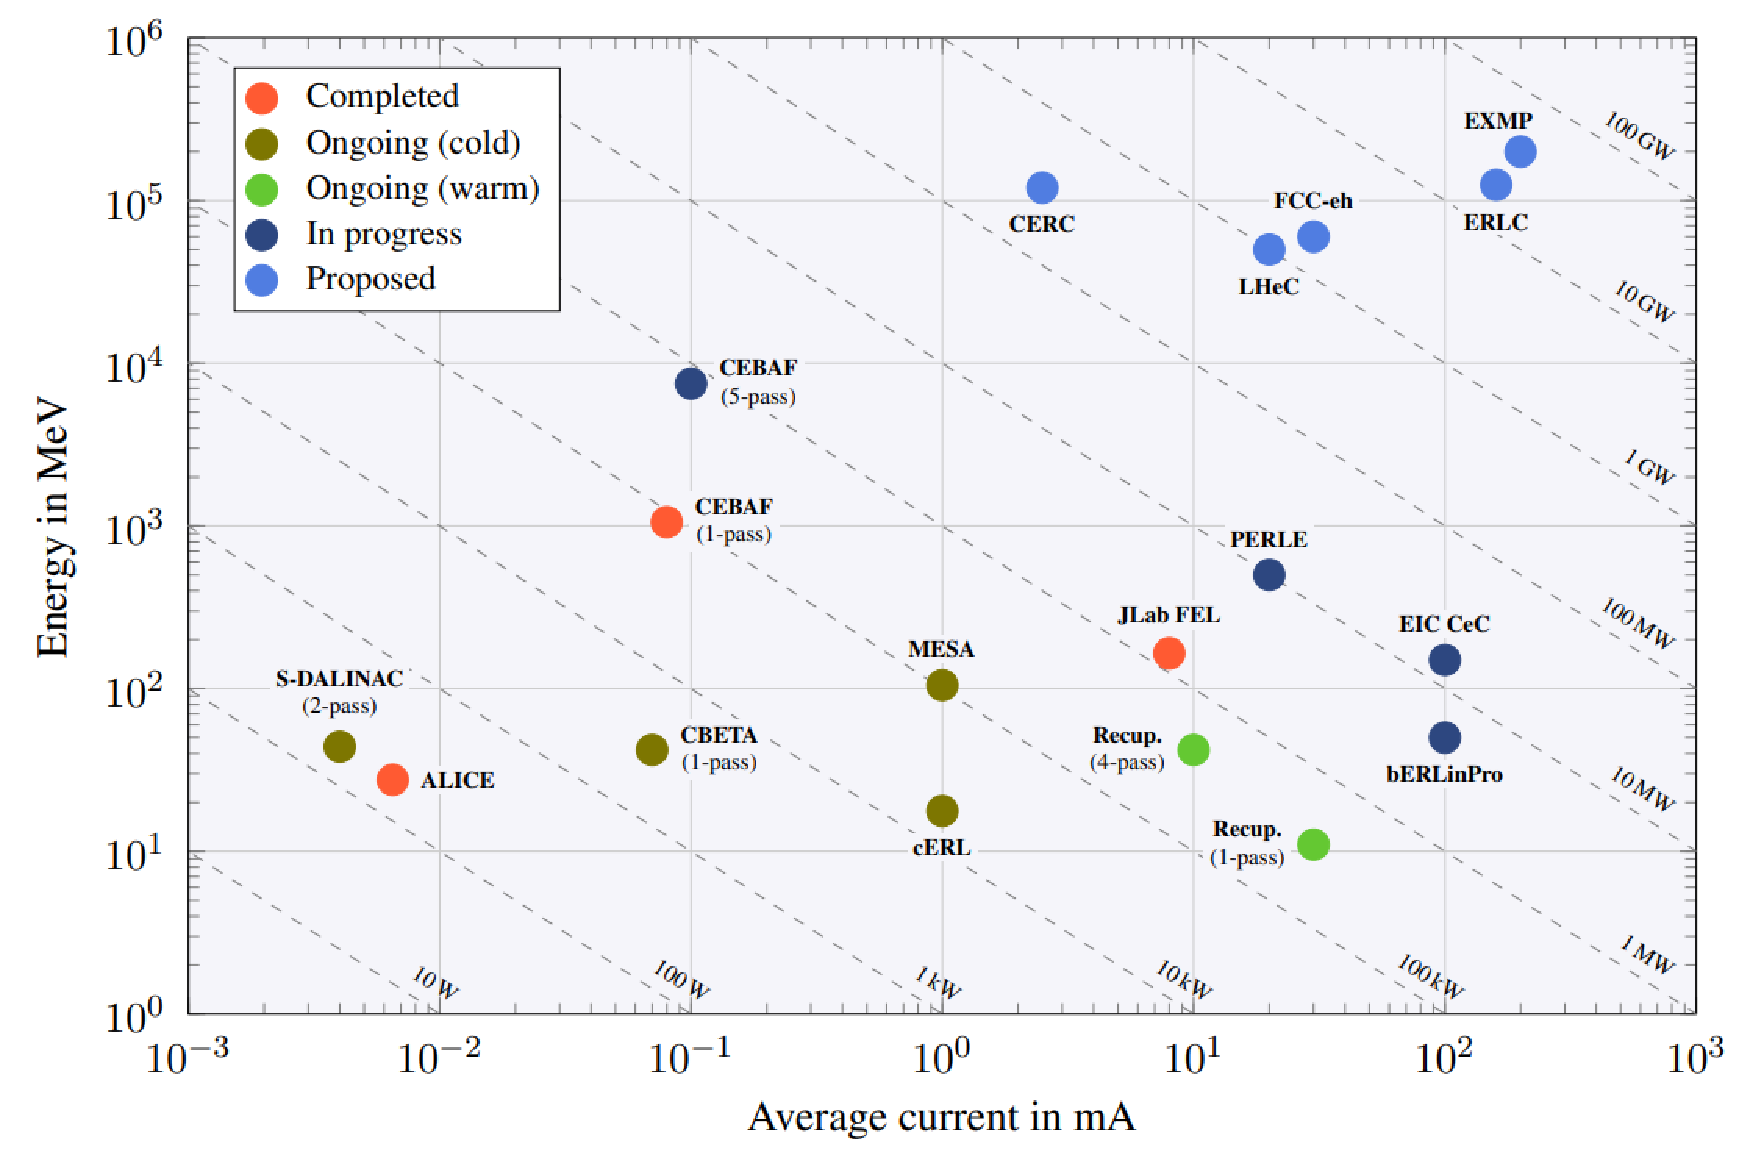
\includegraphics[width=0.9\textwidth]{Figures/CBETA_Multi-Pass_Commissioning/Tennant_ERL_Landscape.pdf}
\caption{The landscape of past, present and proposed ERL projects. Lines show the corresponding average electron beam power. Reproduced from the European Strategy for Particle Physics
Accelerator Research and Development Roadmap \cite{adolphsen2022european}.}
\label{fig:ERL_Landscape}
\end{figure}

The bERLinPro ERL is a single turn ERL which aims to demonstrate high current operation of an ERL with a maximum average beam current of 100~\si{\milli\ampere} at 50~\si{\mega\electronvolt} electron beam energy \cite{kuske2012conceptual,neumann2018berlinpro}. A normalised transverse emittance of 1~\si{\milli\meter}--\si{\milli\radian} with a 2~\si{\pico\second} bunch duration is proposed, which would be the highest brightness electron beam produced in an ERL. However, commissioning of the bERLinPro ERL has been stalled by damage to the main linac cryomodule \cite{neumann2018berlinpro}. Many obstacles to high average current operation in ERLs exist, as explained in Section~\ref{sec:high_current_ERL}, such as coherent synchrotron radiation production, beam breakup instability (BBU) and beam halo which are an active area of study for all ERL projects. BBU and beam halo are a particular focus of studies for bERLinPro \cite{neumann2012status,hwang2019first}.

The proposed ER@CEBAF experiment aims to build upon the previous demonstration of single turn energy recovery at CEBAF \cite{bogacz2003cebaf} discussed earlier with a 5-turn energy recovery linac demonstration. ER@CEBAF aims to extend the operation of an ERL to higher electron energies with a maximum electron energy of 7.5~\si{\giga\electronvolt} \cite{bogacz2016er,meot2016er}. Attaining high electron energies with a reduced length accelerating section is the main advantage of a multi-turn ERL over single turn ERLs because accelerating electron beams to very high energy ($E_{e} < 100$'s~\si{\giga\electronvolt}) with a single-use (traversed once) accelerating section would be prohibitive in size and cost of RF components. Therefore, ER@CEBAF is a necessary demonstrator for future ERL based collider projects such as the LHeC electron--positron collider \cite{valloni2013strawman,bruning2019exploring,holzer2021accelerator} which require very high energies (10's-100's~\si{\giga\electronvolt}). The impact of the synchrotron radiation losses upon the beam dynamics of an ERL for a high energy ERL would be challenging. Consequently, the ER@CEBAF project, with a 7.5~\si{\giga\electronvolt} electron beam energy, could allow for study of synchrotron losses upon momentum acceptance in the re-circulating beam transport optics \cite{adolphsen2022european}.  

PERLE: powerful energy recovery linac for experiments is the highest average electron beam power multi-turn ERL project currently being constructed, with an electron beam energy of 500~\si{\mega\electronvolt} and average electron beam current of 20~\si{\milli\ampere} ($P = 10$~\si{\mega\watt}) \cite{angal2018perle,bogacz2021perle}. PERLE -- a three turn common transport ERL, where accelerating and decelerating electron beams are transported in the same beamline, is designed to provide a moderate energy, moderate current demonstration toward the proposed LHeC ERL project \cite{valloni2013strawman,bruning2019exploring,holzer2021accelerator}. Important ERL topics studied at PERLE will include handling a high average beam current, CW operation, low electron beam energy spread and emittance at an interaction point (IP) \cite{adolphsen2022european} necessary toward future colliders. To achieve a high average electron beam current PERLE utilises a high bunch charge of 500~\si{\pico\coulomb} \cite{hounsell2021optimization}, a factor $\sim3$ higher than previously demonstrated in an SRF ERL at the upgraded JLab FEL \cite{neil2006jlab}. The PERLE ERL is designed with an integrated final focus system which with 500~\si{\mega\electronvolt} electron bunches makes PERLE an ideal driver of an ICS source \cite{adolphsen2022european}; using an IR laser (Nd:YAG $\lambda=1064~\si{\nano\meter}$) PERLE is capable of generating up to 4.45~\si{\mega\electronvolt} $\gamma$-rays.      

%Multi-turn ERLs in particular are a good choice for design of a light source because, as previously demonstrated, multi-turn ERLs can deliver high average electron beam power (\si{\mega\watt}-scale) with small emittances ($\epsilon_{n} < 1$~\si{\milli\meter}) and short bunch lengths (\si{\pico\second}-scale) which constitute high brightness electron beams. In addition, multiple re-circulations allows for higher energy electron beams necessary for small wavelength photon generation to be produced in a compact footprint, without an expensive high power accelerating section. Hence, multi-turn ERLs are investigated as drivers of light sources within this thesis.  

\section{Synchrotron Radiation Production}
\label{sec:synchrotron_radiation_intro}

Synchrotron radiation is the electromagnetic radiation emitted by a relativistically-moving charged particle when deflected by a magnetic field. The magnetic field does no work upon the charged particle but the deflection causes a transverse acceleration and consequently the emission of radiation. In the rest frame of the charged particle, the emission of radiation is isotropic, described in more detail in Section~\ref{sec:radiation_accelerated_charge}; when Lorentz transformed into the laboratory frame the radiation is emitted in the direction of the moving charge into a cone of angle $\theta = 1/\gamma$ (Lorentz factor $\gamma$) with the radiation preferentially emitted in the forward direction, as shown in Fig.~\ref{fig:synchrotron_radiation_diagram}.
\begin{figure}[!h]
\centering
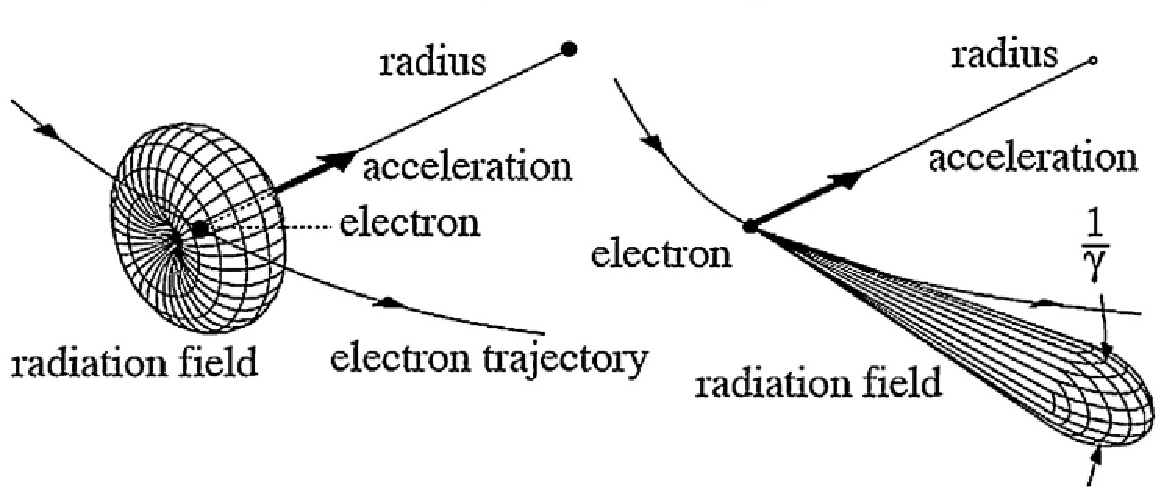
\includegraphics[width=0.8\textwidth]{Figures/Introduction/Synchrotron_Radiation_Diagram.pdf}
\caption{Diagram of the emitted radiation produced by a charged particle deflected by a dipole magnetic field causing the electrons to traverse a curved trajectory. Reproduced and modified from Eberhardt \cite{eberhardt2015synchrotron}. Left: Cyclotron radiation produced by a non-relativistic charged particle. Right: Synchrotron radiation produced by a relativistically-moving charged particle. As observed in the laboratory frame, radiation is produced into an elongated cone, with opening angle $\theta = 1/\gamma$.}
\label{fig:synchrotron_radiation_diagram}
\end{figure}
The power of the emitted radiation from a single charged particle is given by the Larmor formula \cite{larmor1897lxiii}, which can be modified assuming a charge orbits in a circle of bending radius $\rho$ (as in a circular accelerator), to become
\begin{equation}
P = \frac{q^{2}a^{2}\gamma^{4}}{6\pi\epsilon_{0}c^{3}} = \frac{q^{2}c\beta^{4}\gamma^{4}}{6\pi\epsilon_{0}\rho^{2}},
\label{eq:synchrotron_radiation_power}    
\end{equation}
where $q$ is the charge of the particle, $a$ the acceleration due to the magnetic field and $\epsilon_{0}$ is the permittivity of free space. $P \propto \gamma^{4}$ because $a = d^{2}x/dt^{2}$ and the displacement of the charged particle $x$ is Lorentz contracted to $x/\gamma$ such that a factor $\gamma^{2}$ arises due to each acceleration term. Consequently, high energy particles emit large powers of radiation and a particle beam with large average current (containing many electrons $N_{e}\sim 10^{18}$) is capable of producing a high power photon beam ($P_{\mathrm{tot}}=N_{e}P$). To an external observer, synchrotron radiation appears pulsed in nature because it is emitted from a moving particle on a curved trajectory into a $1/\gamma$ cone and the pulse length $\tau$ is shortened by Lorentz contraction ($\tau \propto 1/\gamma$). Since the radiation appears pulsed it must contain a wide range of frequency components \cite{appleby2020science}.  

The critical energy of a synchrotron radiation source is defined as the photon energy at which half the radiation power is produced i.e. half of the radiation is produced with photon energies higher or lower than the critical energy, which is given by
\begin{equation}
E_{\mathrm{crit}} = \frac{3}{2}\frac{\hbar c\gamma^{3}}{\rho}.
\label{eq:synchrotron_critical_energy}    
\end{equation}
Since the power of the synchrotron radiation below the critical energy is equal to that above it, the number of low energy photons produced by a synchrotron radiation source must be much larger. Therefore, we find the average photon energy is given by
\begin{equation}
\langle E_{\gamma} \rangle = \frac{h\gamma^{2}qB}{4\pi m_{e}c^{2}} \approx \frac{8\sqrt{3}}{45}E_{\mathrm{crit}}.
\label{eq:synchrotron_average_energy}    
\end{equation}
A diagram of a typical synchrotron radiation spectrum is shown in Fig.~\ref{fig:synchrotron_spectrum} where the photon flux increases toward the critical energy, with a sharp cut-off in flux past the critical energy (Eq.~\ref{eq:synchrotron_critical_energy}).
\begin{figure}[!h]
\centering
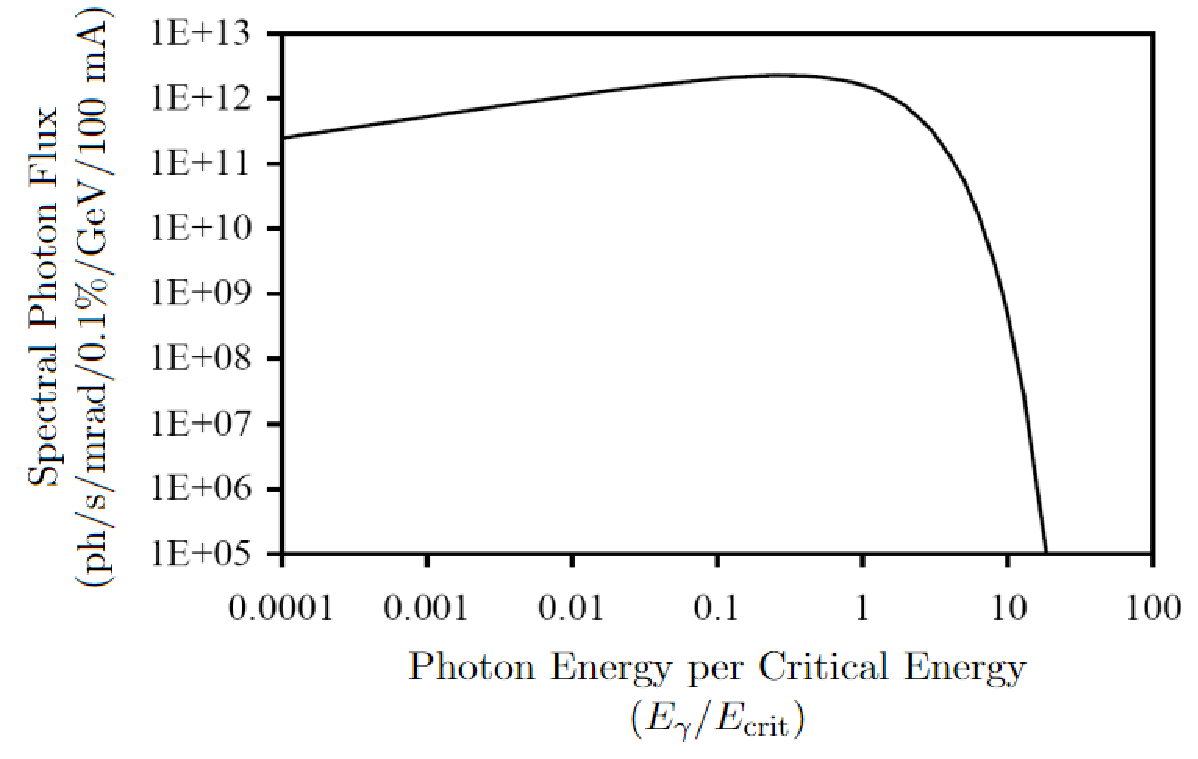
\includegraphics[width=0.7\textwidth]{Figures/Introduction/synchrotron_radiation_spectrum.pdf}
\caption{Typical spectrum of spectral flux against photon energy for synchrotron radiation production. The average photon energy is typically much lower than the critical energy -- the photon energy where half the synchrotron radiation power is emitted below and above this energy. The photon spectrum is continuous with a high flux of photons produced until a sharp cut-off at high energy, above the critical energy of the synchrotron source. Reproduced from Clarke \cite{clarke2016undulators}.}
\label{fig:synchrotron_spectrum}
\end{figure}

Electrons are typically used in laboratory sources of synchrotron radiation because of their small mass in comparison to other particles, such as protons, which means $\gamma$ can be made large and high radiation powers can be generated (Eq.~\ref{eq:synchrotron_radiation_power}). A large Lorentz factor also means that the radiation is directed into a more narrow cone, which is advantageous because the generated radiation can be more readily guided to a downstream experiment. For example, consider the DIAMOND light source \cite{materlik2015diamond}, where a 300~\si{\milli\ampere} average current electron beam with kinetic energy of 3~\si{\giga\electronvolt} orbits the 561.36~\si{\meter} circumference storage ring with dipoles of bending radii $\rho = 7.1$~\si{\meter}, photons are emitted with a total power of 3.81~\si{\mega\watt}, a flux of $9\times 10^{18}$~ph/\si{\second} and a critical energy of 8.46~\si{\kilo\electronvolt}.   

\subsection{Synchrotron Radiation Sources}

Artificially-produced synchrotron radiation was first observed in 1947 at the GE synchrotron, New York, USA \cite{elder1948radiation} and the first systematic description of synchrotron radiation was published by Schwinger in 1949 \cite{schwinger1949classical}. The 70~\si{\mega\electronvolt} GE synchrotron, with bending radius of 0.293~\si{\meter}, produced visible light with a critical energy of $E_{\mathrm{crit}} = 2.65~\si{\electronvolt}$ ($\lambda = 467$~\si{\nano\meter}). The first dedicated accelerator for production of synchrotron radiation was Tantalus I \cite{rowe1973tantalus}, first operated in 1968. Tantalus I demonstrated the utility of synchrotron radiation facilities because they are capable of producing shorter wavelengths ($\lambda < 110$~\si{\nano\meter}) of radiation at higher intensities than previously used continuum radiation sources \cite{rowe1973tantalus}. For example, Tantalus I is capable of producing radiation with a critical energy of 48.6~\si{\electronvolt} ($\lambda = 25.6$~\si{\nano\meter}) and is also capable of high intensities as a total of $8.98\times 10^{18}$~ph/\si{\second} are produced.  

% why is it useful in comparsion to other sources
Synchrotron radiation sources are useful experimentally, particularly at x-ray wavelengths, because the wavelength is tunable via the electron energy, short duration radiation (picosecond-scale) can be produced and significantly higher x-ray fluxes are produced than in conventional bremsstrahlung generation. Advantages of x-ray synchrotron radiation were first demonstrated by the first dedicated x-ray Synchrotron Radiation Source (SRS) at Daresbury \cite{munro2019fifty,robinson1981experiments}, which is shown in Fig.~\ref{fig:daresbury_SRS_diagram}. Modern synchrotrons, for example the SPring-8 synchrotron radiation source, have a maximum average brilliance of $10^{20}$~ph/\si{\second} \si{\milli\meter}$^{2}$--\si{\milli\radian}$^{2}$ 0.1\% BW \cite{spring8beamlines} and are for example capable of producing x-ray pulses with a 32~\si{\pico\second} duration at 14~\si{\kilo\electronvolt} \cite{tanaka2001field}. Modern bremsstrahlung based x-ray tubes, typically used in medicine, have an average brilliance of around $10^{10}$~ph/\si{\second} \si{\milli\meter}$^{2}$--\si{\milli\radian}$^{2}$ 0.1\% BW and a 2~\si{\milli\second} pulse duration \cite{behling2018diagnostic}.
Emission angles $\theta$ of synchrotron radiation are also smaller than bremmstrahlung because the electron beam energy for x-ray production in synchrotrons is larger ($E_{e,\mathrm{synch}}\sim$\si{\giga\electronvolt}) than in bremsstrahlung ($E_{e,\si{brem}}\sim$\si{\mega\electronvolt}) and $\theta \propto 1/\gamma$. For example, an 8~\si{\giga\electronvolt} electron beam from an x-ray synchrotron creates a photon beam with emission angle $\sim 64$~\si{\micro\radian}, producing a small radiation spot size downstream on-sample; at a 100~\si{\meter} source to detector distance the spot size is 112~\si{\micro\meter}.        
\begin{figure}[!h]
\centering
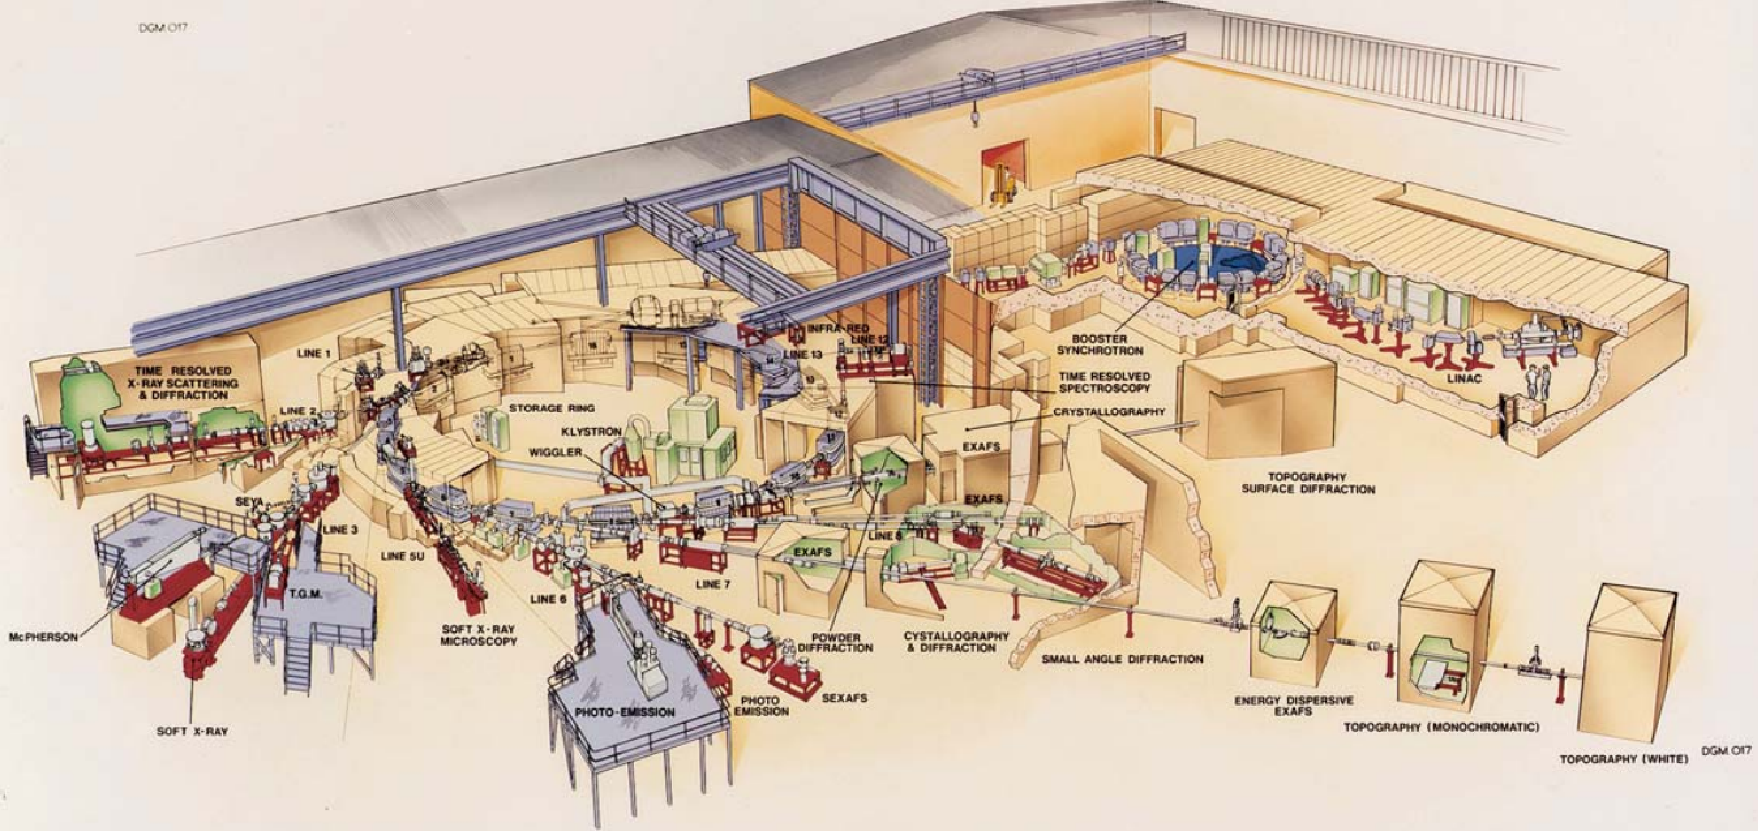
\includegraphics[width=\textwidth]{Figures/Introduction/Daresbury_SRS.pdf}
\caption{Schematic of the Synchrotron Radiation Source facility previously built at Daresbury Laboratory. Electron bunches were produced and accelerated to 5~\si{\mega\electronvolt} by an electron gun, a short linac then accelerated the electrons to 12~\si{\mega\electronvolt} where they enter a 600~\si{\mega\electronvolt} synchrotron booster ring which accelerates the electrons to 2~\si{\giga\electronvolt} for use in the synchrotron light source storage ring. Many beamlines with a varied experimental station design are incorporated to utilise the synchrotron radiation produced from the 2~\si{\giga\electronvolt} electron beam. Reproduced from Rossman et al\cite{rossmann2001international}.}
\label{fig:daresbury_SRS_diagram}
\end{figure}

% Monochromation + why we want brilliance not flux
High brilliance is desired by many synchrotron facility users, such as those conducting spectroscopy and crystallography experiments, because monochromation (i.e. selection of a small energy range or bandwidth) of the synchrotron radiation is required. Bragg diffraction from perfect (defectless) crystals is typically used to monochromate synchrotron radiation as the diffraction angle is wavelength dependent such that a narrow bandwidth can be selected via collimation or optics post monochromation. Further details on monochromation of synchrotron radiation are explained by Caciuffo et al \cite{caciuffo1987monochromators}. A small radiation spot size and angular divergence upon the monochromator is required so the radiation pulse impinges on the monochromator with similar angle irrespective of position in the radiation pulse. Therefore, maximising the synchrotron radiation flux to the monochromator -- dependent on radiation pulse spot size and divergence -- is ideal for synchrotron radiation users, and brilliance is a measure of this. Brilliance of the produced radiation can only be improved via improvements in the electron beam -- the source of the radiation -- such as decreasing the emittance. Therefore, storage rings were designed with electron beam optics to reduce emittance growth, such as the double bend achromat design proposed by Chasman and Green \cite{chasman1975preliminary} (see Section~\ref{sec:achromats}).          

\subsection{Insertion Devices}

% 3rd Generation light sources
% undulators + wigglers 
% GeV scale km circumference machines
Synchrotron radiation facilities were advanced by the emergence of lower emittance designs, higher electron beam energies and the advent of insertion devices such as wigglers and undulators -- with these advancements the synchrotron radiation sources are termed 3rd generation light sources. Insertion devices are typically a series of magnets placed between the dipole bending magnets in a synchrotron, and the insertion devices considered here are designed to increase and modify the synchrotron radiation output. 

The simplest insertion device is a wavelength shifter, where a high field magnet is contained within the straight section between two bending magnets, as shown in Fig.~\ref{fig:wavelength_shifter_wiggler}. A wavelength shifter varies the flux -- energy spectrum (see Fig.~\ref{fig:synchrotron_spectrum}) of the synchrotron radiation by modifying the critical energy (Eq.~\ref{eq:synchrotron_critical_energy}) since $E_{\mathrm{crit}} \propto 1/\rho \propto B$ and increasing the power of the emitted radiation $P \propto 1/\rho^{2} \propto B^{2}$. Superconducting high field magnets are typically used in wavelength shifters, for example the 6~\si{\tesla} SRS wavelength shifter \cite{poole1989second}.   
\begin{figure}[!h]
\centering
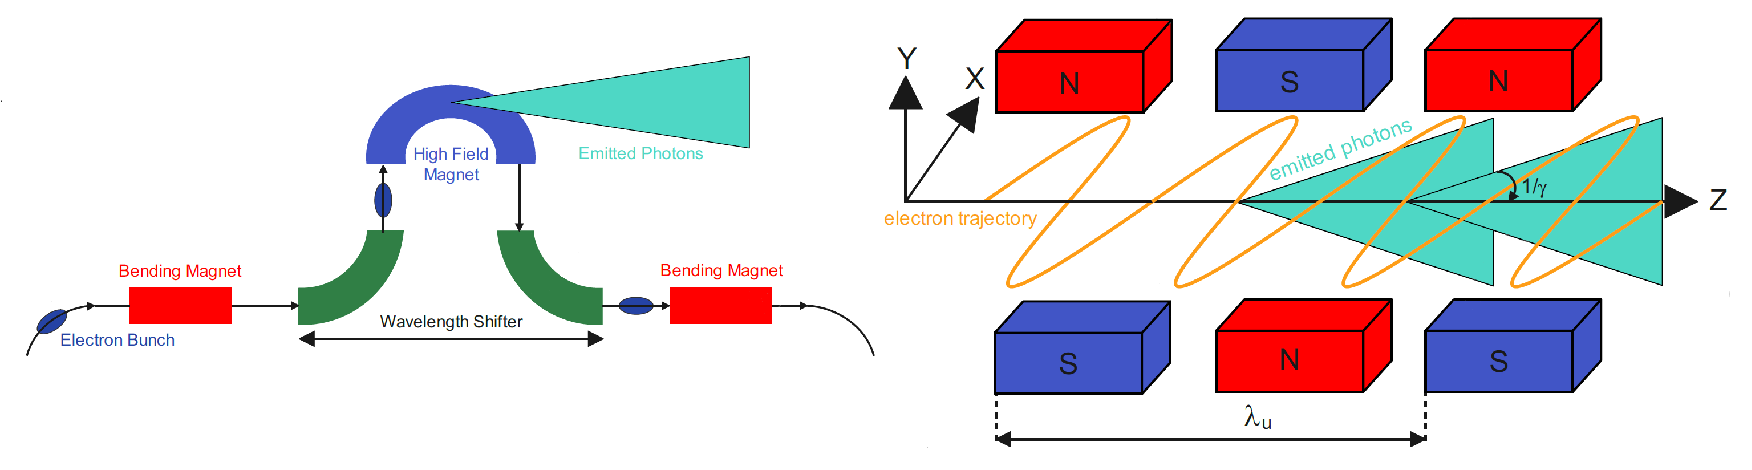
\includegraphics[width=\textwidth]{Figures/Introduction/wavelength_shifter_wiggler.pdf}
\caption{Left: A wavelength shifter is typically imposed between the two dipole bending magnets (red) of a storage ring where a high field magnet (blue) is used to generate synchrotron radiation (turquoise) that is produced parallel to the direction of the electron bunch in the straight. Right: A multipole wiggler consisting of two rows of high-field magnets (typically superconducting) with opposing polarity (north (red), south (blue)) suspended above one another which generates a vertical sinusoidal magnetic field of period $\lambda_{u}$. The strong vertical sinusoidally-varying magnetic field causes the electron trajectory (orange) to oscillate horizontally and generate synchrotron radiation (turquoise) into a cone of angle $\theta = 1/\gamma$. Electrons oscillate with large variation in horizontal position ($x \propto K/\gamma$) therefore cones of consecutively produced synchrotron radiation do not fully overlap. }
\label{fig:wavelength_shifter_wiggler}
\end{figure}

Consider a series of $n$ wavelength shifters placed into the straight which form a periodic series of opposing polarity magnets, such as in the wiggler shown in Fig.~\ref{fig:wavelength_shifter_wiggler}. Each individual wiggler period then acts as an independent source of synchrotron radiation, and since they all emit in the same direction, an observer at the end of the periodic series of magnets would witness a factor $n$ times the flux produced by a single wavelength shifter. A wiggler is advantageous because the critical energy of the photons can be selected independently of the bending magnets by tuning the wiggler magnetic field ($E_{\mathrm{crit}} \propto B$), so photon energy can be tuned to experimental requirements, and the flux available to a user is increased linearly by the number of wiggler periods (wavelength shifters) used.

The trajectory of an electron in a periodic series of alternating polarity magnets, for small angular deflections ($dx/ds \ll 1$, $dy/ds \ll 1$), is given by the equations of motion
\begin{align}
\frac{d^{2}x}{ds^{2}} &= \frac{e}{\gamma m_{e}c}\left(B_{y}-\frac{dy}{ds}B_{s}\right), & \frac{d^{2}y}{ds^{2}} = \frac{e}{\gamma m_{e}c}\left(\frac{dx}{ds}B_{s}-B_{x}\right), 
\label{eq:undulator_equations_of_motion}    
\end{align}
where $B_{x},~B_{y},~B_{s}$ are the horizontal, vertical and longitudinal components of the wiggler magnetic field respectively. If we consider a periodic series of alternating polarity magnets with only a vertical magnetic component, as shown for the wiggler in Fig.~\ref{fig:wavelength_shifter_wiggler}, which deflects the electron horizontally, the equations of motion become
\begin{align}
\frac{d^{2}x}{ds^{2}} &= \frac{eB_{y}}{\gamma m_{e}c}, & \frac{d^{2}y}{ds^{2}} &= 0.
\label{eq:planar_undulator_equations_of_motion}    
\end{align}
We also assume that the magnetic field is sinusoidal form with a period $\lambda_{u}$
\begin{equation}
B_{y}\left(s\right) = -B_{0}\sin\left(\frac{2\pi s}{\lambda_{u}}\right),
\label{eq:wiggler_magnetic_field}    
\end{equation}
where $B_{0}$ is the amplitude of the magnetic field. Consequently, the equation of motion and the angular deflection $dx/ds$ for a horizontally deflecting magnetic field become
\begin{align}
\frac{d^{2}x}{ds^{2}} &= -\frac{e}{\gamma m_{e}c}B_{0}\sin\left(\frac{2\pi s}{\lambda_{u}}\right), \\
\frac{dx}{ds} &= \frac{e}{\gamma m_{e}c}B_{0}\frac{\lambda_{u}}{2\pi}\cos\left(\frac{2\pi s}{\lambda_{u}}\right).
\label{eq:undulator_eq_of_motion_deflection}
\end{align}
The deflection parameter $K$ is defined as the maximum angular deflection ($dx/ds$) of the electron within a series of alternating polarity magnets and is given by
\begin{equation}
K = \frac{B_{0}e\lambda_{u}}{2\pi m_{e}c}.
\label{eq:deflection_parameter}    
\end{equation}
The horizontal position of the electron is therefore given by 
\begin{equation}
x\left(s\right) = \frac{K}{\gamma}\frac{\lambda_{u}}{2\pi}\sin\left(\frac{2\pi s}{\lambda_{u}}\right).
\label{eq:x_electron_undulator}    
\end{equation}

For deflection parameters $K \gg 1$, we defined the periodic series of alternating polarity magnets as a wiggler because these have strong magnetic fields. The horizontal deflection of the electron beam (Eq.~\ref{eq:x_electron_undulator}) means the electron position $\propto K/\gamma$ whereas the synchrotron radiation is emitted into a cone of $\theta \propto 1/\gamma$ and therefore, since $K \gg 1$, the produced synchrotron radiation from subsequent periods does not overlap much. Hence, the radiation from each wiggler period in a wiggler is independent.

However, an undulator is defined to have a small deflection parameter $K < 1$, where the synchrotron radiation produced from each period (undulator period $\lambda_{u}$) constructively interferes. These are often constructed from permanent magnets, for example the many permanent magnet undulators at the DIAMOND light source \cite{materlik2015diamond}, and a diagram of an undulator is shown in Fig.~\ref{fig:planar_undulator_diagram}. A deflection parameter $K < 1$ ensures the electron position varies by a small amount such that synchrotron radiation produced from consecutive wavelength shifters into an angular cone of $1/\gamma$ can overlap. Assuming a planar undulator, as shown in Fig.~\ref{fig:planar_undulator_diagram}, with only a vertical magnetic field, the transverse relativistic velocities of the electron in the undulator are given by
\begin{align}
\beta_{x} &= \frac{K}{\gamma}\cos\left(\frac{2\pi s}{\lambda_{u}}\right), & \beta_{y} &= 0,
\label{eq:transverse_undulator_velocity}    
\end{align}
and the longitudinal velocity $\beta_{s}$ becomes
\begin{equation}
\beta_{s}^{2} = \beta^{2}-\frac{K^{2}}{\gamma^{2}}\cos^{2}\left(\frac{2\pi s}{\lambda_{u}}\right),
\label{eq:longitudinal_undulator_velocity}
\end{equation}
where $\beta$ is the Lorentz speed factor. Consequently, there is a phase slip from the electron with respect the the emitted synchrotron radiation.
\begin{figure}[!h]
\centering
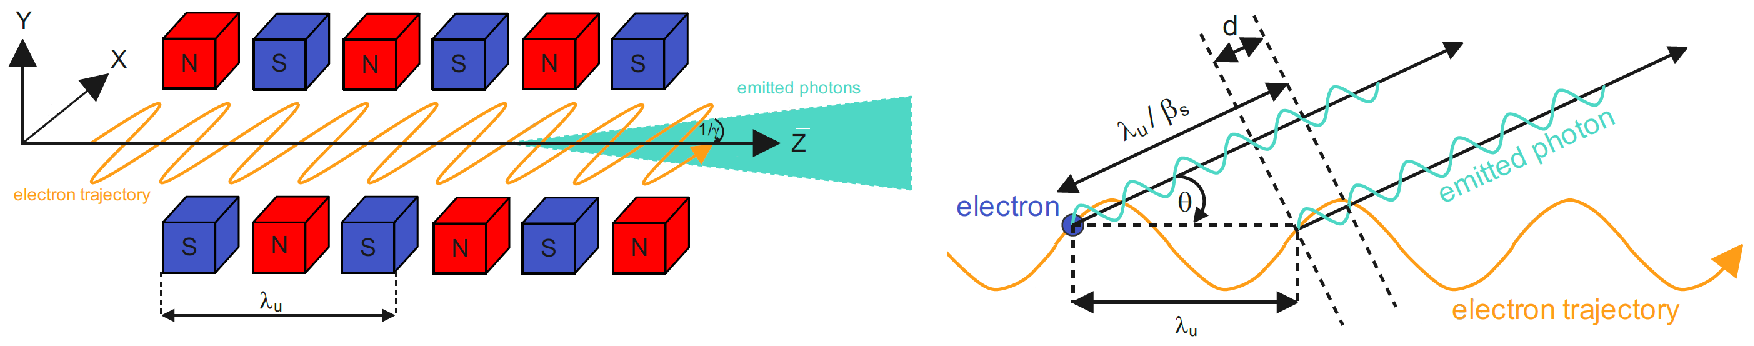
\includegraphics[width=\textwidth]{Figures/Introduction/undulator_and_interference.pdf}
\caption{Left: Planar undulator composed of two rows of several opposing polarity (north (red), south (blue)) magnets (typically permanent magnets) suspended about one another, which generate a vertical sinusoidally-varying magnetic field with period $\lambda_{u}$. The vertical magnetic field causes the electron beam to oscillate transversely and emit synchrotron radiation (turquoise). Right: Interference of the emitted synchrotron radiation (turquoise) from consecutive undulator periods $\lambda_{u}$. As the electron trajectory (orange) oscillates in an undulator it traverses an undulator period in time $t= \lambda_{u}/c\hat{\beta_{s}}$, whereas the wavefront of the emitted synchrotron radiation traverses an undulator period in time $t=\lambda_{u}/\hat{\beta_{s}}$. However, synchrotron radiation that is produced from consecutive undulator periods can constructively interfere is the distance $d$ between each emission is an integer number of wavelengths.}
\label{fig:planar_undulator_diagram}
\end{figure}

Constructive interference of the consecutively produced synchrotron radiation can therefore occur if the electron longitudinal position slips back an integer number of emitted wavelengths with respect to the emitted synchrotron radiation. As shown in Fig.~\ref{fig:planar_undulator_diagram}, the separation $d$ between consecutively emitted cones of synchrotron radiation in an undulator is 
\begin{equation}
d = \frac{\lambda_{u}}{\hat{\beta_{s}}} - \lambda_{u}\cos\theta,
\label{eq:undulator_constructive_interference}    
\end{equation}
such that the consecutively emitted cones of synchrotron radiation constructively interfere when $d=n\lambda$, with $\lambda$ the wavelength of the emitted radiation. Hence, the undulator equation becomes
\begin{equation}
\lambda = \frac{\lambda_{u}}{2n\gamma^{2}}\left(1+\frac{K^{2}}{2}+\gamma^{2}\theta^{2}\right),
\label{eq:undulator_equation}    
\end{equation}
where $\theta$ is the angle of emission and $n$ is the harmonic number. Harmonics of the radiation can be produced with shorter wavelengths when $n = 2,~3,~4$ etc. however, only odd harmonics of radiation are produced on-axis by an undulator. For example, consider a typical undulator with period $\lambda_{u} = 0.1$~\si{\meter} and deflection parameter $K = 0.7$ traversed by an electron energy of 3~\si{\giga\electronvolt} produces photons on-axis ($\theta = 0$) in the fundamental harmonic ($n=1$) with wavelength $\lambda = 3.61$~\si{\nano\meter} ($E_{\gamma} = 344$~\si{\electronvolt}). The undulator equation (Eq.~\ref{eq:undulator_equation}) shows the energy of the emitted photon $E_{\gamma} \propto \gamma^{2}$, so high photon energies require high energy electrons and $E_{\gamma} \propto 1/B$ so increasing the magnet strength produces longer wavelength photons. 

The first undulator was demonstrated on a linac in 1953 at Stanford university \cite{motz1953experiments}, then subsequently demonstrated in straight sections of the LPI RAS synchrotron light source in 1977 \cite{bessonov2010light}. However, the magnet density of undulators with relatively strong fields $\sim1$\si{\tesla} and alternating polarity meant undulators could not be practically implemented until the design of permanent magnet undulators by Hallbach et al \cite{halbach1983permanent}. Undulators were then widely utilised in synchrotron sources. Similarly, wigglers were demonstrated in 1979 \cite{berndt1979initial} but became favoured devices for synchrotron production at the shortest wavelengths through use of high field superconducting magnets. For example, a 10~\si{\tesla} wiggler was demonstrated with an 8~\si{\giga\electronvolt} electron beam at SPring-8, generating \si{\mega\electronvolt}-scale $\gamma$-rays \cite{soutome2003generation}.    

\subsection{Free Electron Lasers}

Consider a relativistic bunch of electrons with bunch length $\sigma_{z}$ traversing an undulator with undulator period $\lambda_{u}$. Typically, electron bunch lengths are on the order of $\sim$1--10's~\si{\milli\meter}'s and undulator periods are 1--10's~\si{\centi\meter}'s long. In the rest frame of the electron bunch, the bunch length is $\gamma\sigma_{z}$ and the undulator period is $\lambda_{u}/\gamma$, due to Lorentz contraction between the two frames. Therefore, we find the electron bunch length is far longer $\sigma_{z}\gg \lambda_{u}/\gamma^{2}$; for example, in the SASE1 undulator of EU-XFEL the \textit{rms} bunch length is $\sigma_{z} = 25$~\si{\micro\meter}, the electron beam energy is $E_{e} = 17.5$~\si{\giga\electronvolt} ($\gamma = 34248$) and the undulator period is $\lambda_{u} = 304$~\si{\nano\meter} so the inequality becomes $25~\si{\micro\meter} \gg 304~\si{\nano\meter}$. Hence, in the rest frame individual electrons oscillate with different phases because they are acted upon by different phases of the undulator magnetic field and the output radiation is incoherent.

The total electric field of the oscillating electrons is given by
\begin{equation}
\lvert E_{\mathrm{Tot}}\rvert = \sum_{n=1}^{N}E_{0}\exp\left(i\phi_{n}\right),
\label{eq:undulator_bunch_electric_field}    
\end{equation}
where $E_{0}$ is the electric field due to a single electron and $\phi_{n}$ is the phase of the electric field from the $n$th electron. For incoherent radiation production the electric field becomes \cite{wolski2012fel} % cite andy wolski lectures
\begin{equation}
\lvert E_{\mathrm{Tot}}\rvert = \sqrt{N_{e}}E_{0},
\label{eq:incoherent_electric_field}
\end{equation}
where $N_{e}$ is the number electrons. Consequently, the emitted radiation power varies with electric field and number of electrons as $P \prop E_{\mathrm{tot}}^{2} \prop N_{e}$. However, if all the electrons are oscillating in phase i.e. $\phi_{n}\sim \phi_{0}$ we have coherent radiation production. This occurs when
\begin{equation}
\sigma_{z} \ll \frac{\lambda_{u}}{\gamma^{2}} \approx \lambda,
\label{eq:coherence_condition}
\end{equation}
because then the electron bunch is small in comparison to the oscillating magnetic field and each electron is acted upon by the same magnetic field. We find that $\lambda_{u}/\gamma^{2} \approx \lambda$ due to the undulator equation (Eq.~\ref{eq:undulator_equation}). The coherence condition $\sigma_{z} \ll \lambda$ is difficult to satisfy, as illustrated by the previous EU-XFEL numerical example, since for x-ray radiation production we require sub-angstrom electron bunch lengths. However, when the electrons oscillate in-phase ($\phi_{0}\sim \phi_{n}$) i.e. the coherence condition is satisfied, the total electric field is given by
\begin{equation}
\lvert E_{\mathrm{Tot}}\rvert = N_{e}E_{0},
\label{eq:coherent_electric_field}    
\end{equation}
and the emitted power $P \propto E_{\mathrm{Tot}}^{2} \propto N_{e}^{2}$ \cite{pellegrini2016physics} such that higher photon powers can be achieved with coherent radiation production. When coherent radiation production in an undulator is enabled this is termed lasing as the electron beam acts as a gain medium similar to that of a conventional laser \cite{brau1988free}, hence this radiation production method is known as a free electron laser. 

Free electron lasers take advantage of the increase in emitted power due to coherent radiation production. However, coherent radiation production is only possible with short electron bunches on the order of the emitted radiation wavelength. Achieving this longitudinal distribution can be challenging, but the electron bunch can be microbunched, where the accelerator electron bunch is subdivided into smaller units such that the emission wavelength and electron bunch length match. The required microbunched electron beam longitudinal distribution for free electron lasing can be achieved in numerous ways, but is typically achieved by self amplification by spontaneous emission (SASE) or seeding approaches. These approaches rely upon interaction between the electron bunch and either the incoherent radiation emitted in the undulator or a seed radiation source; two possible approaches are shown in Fig.~\ref{fig:FEL_microbunching}.
\begin{figure}[!h]
\centering
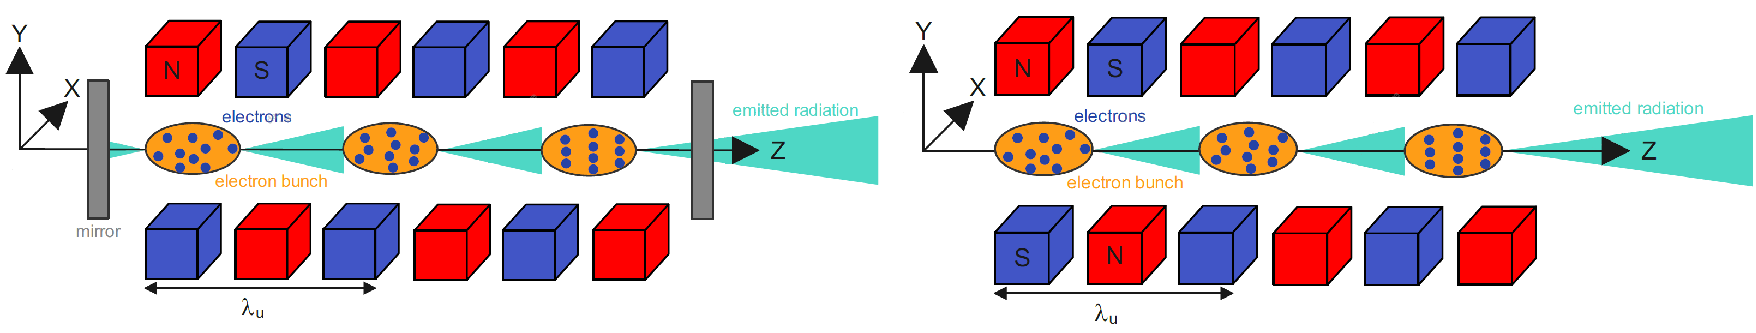
\includegraphics[width=\textwidth]{Figures/Introduction/FELs_microbunching.pdf}
\caption{A series of electron bunches (orange) traverse an undulator. The electrons in the bunch (blue) are typically disordered longitudinally upon entering the undulator, however as the electron bunches propagate through the undulator they emit synchrotron radiation incoherently. The incoherent synchrotron radiation produced from the $n+1$th bunch interacts with the $n$th leading bunch and the self-interaction between the incoherent radiation and the electrons in the $n$th bunch causes microbunching of the electrons for coherent emission. Left: A resonator FEL, which uses a short undulator -- smaller than the distance it would take for microbunching to develop -- and a pair of mirrors (grey) which reflect the synchrotron radiation for further self-interaction with the electron bunches which causes microbunching an coherent emission. Right: A SASE FEL with a long undulator such that microbunching occurs as the electron bunch propagates throughout the undulator. Once the electron bunch is microbunched, coherent synchrotron radiation production occurs. }
\label{fig:FEL_microbunching}
\end{figure}

Self-interaction can also be seeded, by using an initial, often low power, external source of coherent radiation such as a conventional laser which initially microbunches the electron beam \cite{allaria2012highly}. A coherent seed means the produced radiation is also coherent, and avoids the temporal coherence issues associated with SASE methods. Higher harmonics of the initial seeding laser may be used in order to generate higher wavelength radiation. However, seeded FELs are fundamentally limited by a lack of coherent sources beyond the \si{\nano\meter}-scale.

In SASE operation, self-interaction between the electron bunch and the generated undulator radiation causes energy exchange between the incoherent synchrotron radiation produced by the following bunch and the electrons in the leading bunch which, with many electron bunch--radiation field interactions, drives microbunching of the electron bunch \cite{kondratenko1980generating,bonifacio1984collective}. The microbunched electron beam has the required longitudinal distribution and therefore coherent emission occurs. However, temporal coherence is compromised because the SASE process is started randomly from `shot noise' arising from the random distribution of
electron arrival times at the beginning of the FEL interaction region \cite{mcneil2003unified}. The coherence of the SASE output is restricted as a radiation wavefront may propagate through only a fraction of a typical electron bunch as $v_{z} < c$ and therefore many regions of the radiation/electron interaction will be uncorrelated in phase \cite{thompson2010improved} and consequently the temporal coherence of SASE emission is limited. Temporal coherence challenges with SASE can be overcome via monochromating the radiation pulse before it is used to seed lasing. The incoherent undulator radiation is filtered with a monochromator to reduce the large noise bandwidth before the monochromated radiation is re-used to microbunch the electron bunches and, since the noise has been removed by the monochromator, the subsequent synchrotron radiation produced by the undulator has improved temporal coherence. The LCLS x-ray FEL first demonstrated this self-seeding approach to SASE FELs with a diamond monochromator \cite{emma2010first}. However, since incoherent radiation must first be generated before lasing can occur SASE FELs are typically long ($L\sim 100$'s~\si{\meter}).

Self-interaction of the undulator radiation with the electron bunch can also be achieved via use of a small undulator and a series of mirrors, known as an optical cavity \cite{petrillo2012photon}, to circulate the produced radiation for re-interaction, which is termed a resonator FEL. An example of a 2-mirror resonator FEL is shown in Fig.~\ref{fig:FEL_microbunching}. Resonator FELs are limited in power because high power photon beams incident on the re-circulating mirrors can damage the optics. Also, for high energy photons, such as x-rays, mirrors poorly reflect the incoherent synchrotron radiation -- only a small power is reflected -- such that seeding coherent interaction is less feasible. In addition, the temporal coherence issues discussed for SASE are also present because incoherent undulator radiation is used to seed the FEL.

% Seeding - limited by available seeds i.e. no x-ray seeding possible (need initial coherent source)
The first free electron laser was demonstrated at Stanford University in by Deacon et al \cite{deacon1977first} in 1977, with infrared lasing (coherent photon production) at a wavelength of $\lambda = 3.41$~\si{\micro\meter} and 7~\si{\kilo\watt} peak power; the initial Stanford FEL experiment was an example of a seeded FEL. The lowest wavelength seeded FEL demonstrated to date is the FERMI@ELETTRA FEL \cite{allaria2012highly} with a minimum wavelength of $\sim10$~\si{\nano\meter}. Seeded FELs are yet to probe the x-ray regime because they require a seed radiation of the same wavelength as the emitted wavelength. The first x-ray FEL LCLS was first demonstrated in 2010 at SLAC using a SASE approach to produce a minimum wavelength of 1.2~\si{\angstrom}, a sub-picosecond pulse duration (500--10~\si{\femto\second}), a 0.2--0.5\% FWHM bandwidth and up to 40~\si{\giga\watt} peak power \cite{emma2010first}.

\subsection{Comparison of Synchrotron Radiation Sources}

The peak brilliance -- a measure of the photons produced per pulse duration per unit area in phase space within a small 0.1\% energy spread (bandwidth) (see Chapter~\ref{Photon_Production_by_Inverse_Compton_Scattering}) -- of a series of world-leading light sources are shown in Fig.~\ref{fig:light_source_tuning_curves}. Brilliance is often termed brightness, both are identical quantities, however the convention of brightness for electrons and brilliance for photons is used in this thesis. 
\begin{figure}[!h]
\centering
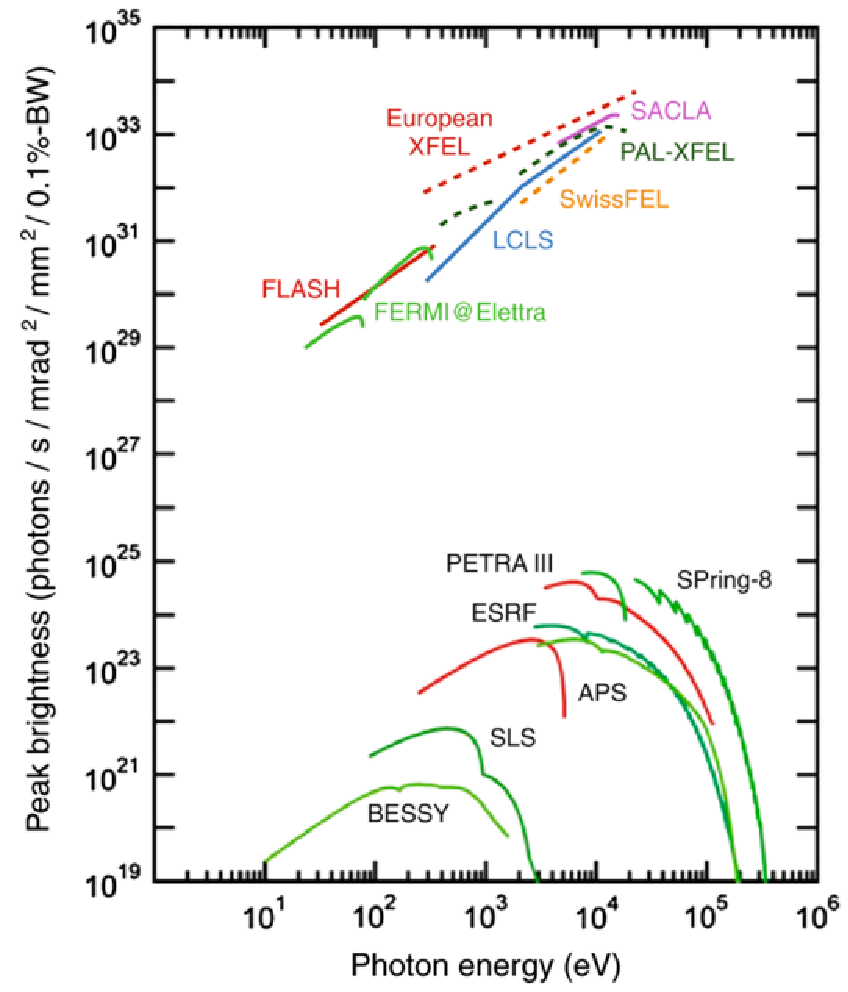
\includegraphics[width=0.6\textwidth]{Figures/Introduction/Light_Source_Brilliance_Energy.pdf}
\caption{Peak brilliance--photon energy tuning curves of a collection of existing x-ray light source facilities, showing both free electron lasers and synchrotron light sources \cite{geloni2017physics}. Note that brilliance is termed brightness here, whilst the two are identical brightness is reserved for discussion of electrons in this thesis. Existing synchrotron radiation sources appear limited in photon energy to $\sim 300$~\si{\kilo\electronvolt}, whilst X-FELs such as the European X-FEL \cite{schneidmiller2011photon} are limited to around 25~\si{\kilo\electronvolt}.}
\label{fig:light_source_tuning_curves}
\end{figure}

Ultimately, as demonstrated in Chapter~\ref{CBETA_Inverse_Compton_Scattering_Source_Design}, practical considerations such as size and magnetic field strength limit synchrotron radiation facilities and free electron lasers to x-ray production with photon energies of $E_{\gamma} < 300~\si{\kilo\electronvolt}$. For development of a $\gamma$-ray source, methods based on synchrotron or undulator radiation fail to produce the \si{\mega\electronvolt}-scale photons desired by nuclear physics experiments \cite{budker2021expanding}. However, synchrotron radiation facilities and FELs are the dominant radiation production methods in the x-ray regime, with unparalleled photon flux and brilliance.  

\section{Bremsstrahlung Radiation Production}
\label{sec:bremsstrahlung}
% Hywels lecture notes give a good brief overview of Brem (in the chapter comments directory) + have the review he gave me
% Duane - Hunt law
% Continuous spectrum - hard to monochromate - why no gamma monochromators?
% High Z good, why? High field for breaking
% bit of history? x-ray generation?

In the bremsstrahlung process a charged particle traverses within the vicinity of atomic nuclei and the strong electric field of the atomic nuclei act on the charged particle causing an acceleration; therefore the particle radiates. A diagram of the bremsstrahlung interaction is shown in Fig.~\ref{fig:brem_intro_diagram}. A more comprehensive description is presented in Section~\ref{sec:bremsstrahlung_comparison} and a full quantum electrodynamic description of bremsstrahlung has been derived by Bethe and Heitler \cite{bethe1934stopping}. A full review of the bremsstrahlung process is beyond the scope of this thesis, and the reader is directed to more comprehensive reviews such as that by Koch and Motz \cite{koch1959bremsstrahlung}. 
\begin{figure}[!h]
\centering
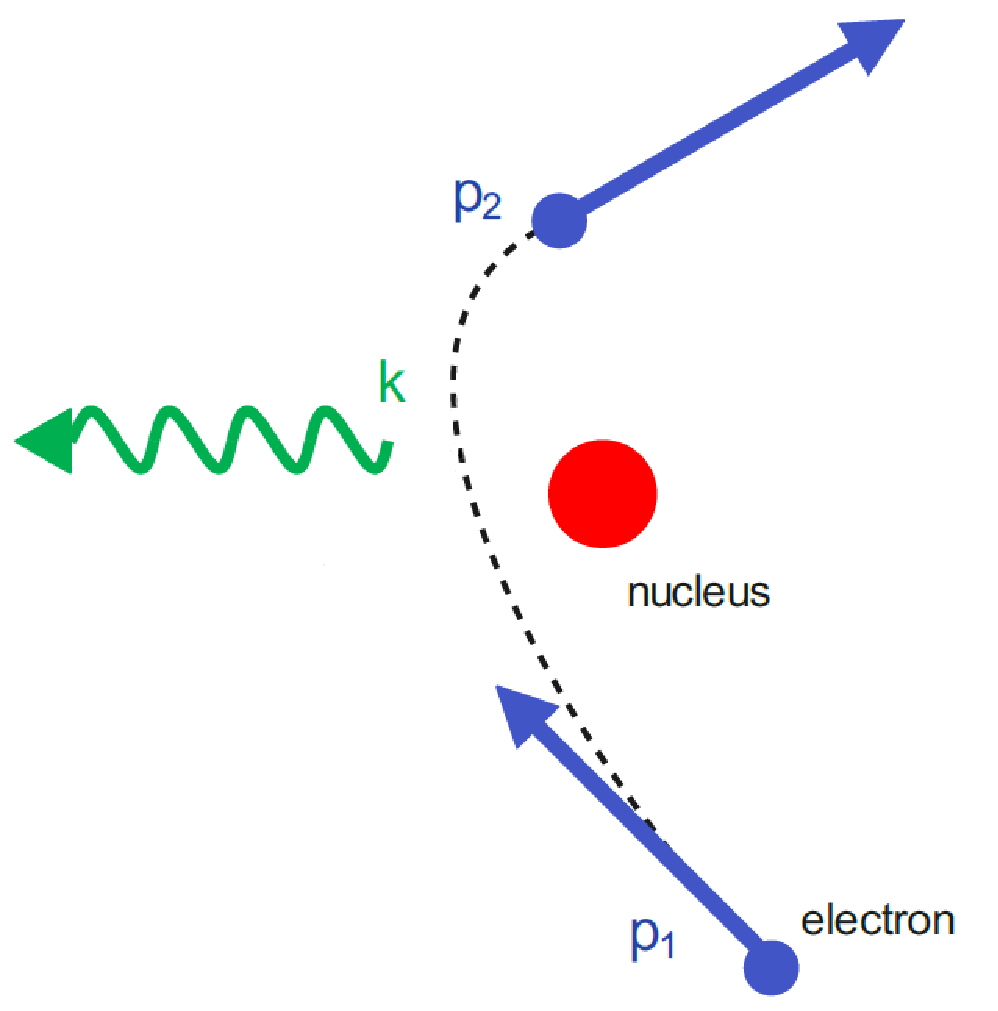
\includegraphics[width=0.6\textwidth]{Figures/Introduction/brem_intro_diagram.pdf}
\caption{Left: Diagram of the bremsstrahlung process where an electron (blue) with momentum $p_{1}$ is bent from its original trajectory by the Coulomb attraction of a nearby nucleus (red) causing the electron to decelerate and therefore radiate. The momentum of the electron is reduced $p_{2} < p_{1}$ and a photon (green) is generated with momentum $\hbar k$, with energy equal to the kinetic energy reduction of the electron.}
\label{fig:brem_intro_diagram}
\end{figure}

Typically, in a bremsstrahlung source a moderate energy electron beam (10--100's~\si{\mega\electronvolt}) is incident upon a dense target of high atomic number $Z$ material (such as tungsten), with photons generated in the direction of the particle beam. The spectrum of radiation produced by a bremsstrahlung interaction is broadband ($0 \leq E_{\gamma} \leq E_{k}$), with the maximum photon frequency $\nu_{\mathrm{max}}$ produced given by the Duane--Hunt law \cite{duane1915proceedings}
\begin{equation}
E_{k}=h\nu_{\mathrm{max}},
\label{eq:duane_hunt_intro}
\end{equation}
where $E_{k}$ is the kinetic energy of the charged particle, $h$ is Planck's constant and $E_{\gamma}=h\nu$ is the generated photon energy. Therefore, with moderate energy \si{\mega\electronvolt}-scale electron beams $\gamma$-rays can be readily generated. When highly relativistic electron beams are used, the resultant photons are produced into an angular cone of opening angle $\theta\sim 1/\gamma$, however simple collimation is insufficient for energy selection because the angle $\theta$ the photon is generated into does not simply correspond to the energy of the generated photon. Monochromation of x-ray radiation is readily carried out, for example with silicon crystals, as explained in Section~\ref{sec:synchrotron_radiation_intro}, but efficient monochromation of $\gamma$-rays has not yet been demonstrated -- currently 2~\si{\mega\electronvolt} $\gamma$-rays have been monochromated with an efficiency of 22\% \cite{jentschel2012gamma}. 

The power of the generated bremsstrahlung radiation increases with increasing atomic number $Z$ because the electric field strength increases as a function of $Z$ ($P \propto Z^{2}$). The density of the target also increases the power of the bremsstrahlung source due to the increased probability of interactions in a thick target since there are more atoms in the target ($P \propto N_{\mathrm{atom}}$). However, the flux of a bremsstrahlung source can also be increased via maximising the electron beam current impinging upon the target, though this causes heating of the target material and thus for high flux bremsstrahlung targets (converters) water cooling is required \cite{auslender2004bremsstrahlung}. High fluxes of both x-rays and $\gamma$-rays are available using a high-$Z$ water cooled target, for example the Advanced Rare Isotope Laboratory (ARIEL) electron linac project \cite{dilling2013ariel} where a 50~\si{\mega\electronvolt} electron linac with an average beam current of 10~\si{\milli\ampere} and a tungsten ($Z = 74$) target are used to generate up to $10^{14}$ $\gamma$-rays per second \cite{lebois2011simulations}. A diagram of the ARIEL electron linac bremsstrahlung source is shown in Fig.~\ref{fig:ARIEL_facility}.
\begin{figure}[!h]
\centering
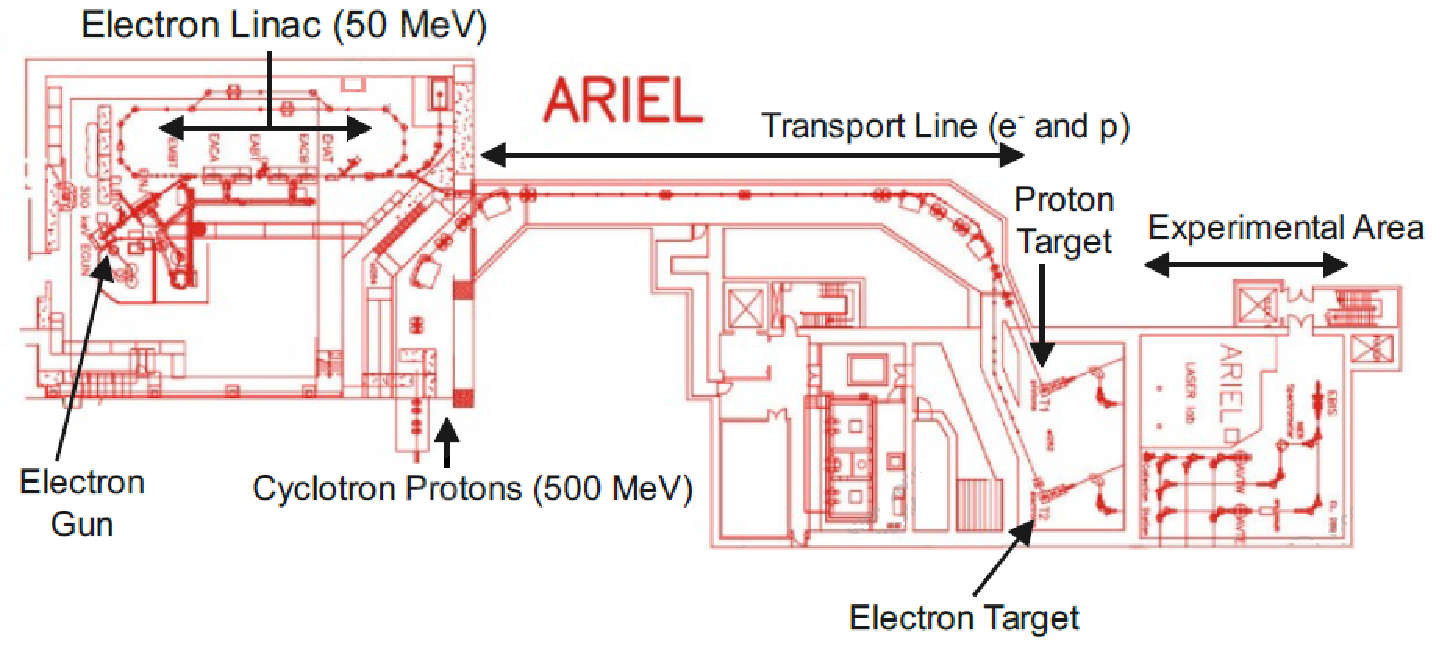
\includegraphics[width=0.9\textwidth]{Figures/Introduction/ARIEL_facility_fixed.pdf}
\caption{The ARIEL facility \cite{dilling2013ariel}. Electrons in ARIEL are accelerated by a 50~\si{\mega\electronvolt} electron linac with an average beam current of 10~\si{\milli\ampere} and transported via a transport line to a bremsstrahlung target station where $\sim 10^{14}$~ph/\si{\second} are generated for use in the experimental area. ARIEL also has the capability to transport $\sim500$~\si{\mega\electronvolt} protons from a cyclotron (not shown) using the same transport line to a proton target for generation of rare isotopes.}
\label{fig:ARIEL_facility}
\end{figure}

Bremsstrahlung radiation production is widely used for example in x-ray production for medical purposes, from the first medical x-ray usage by Jones and Lodge in 1896 \cite{jones1896discovery} to today's computed tomography systems \cite{hounsfield1973computerized,cormack1963representation,cormack1964representation} and modern radiography, with higher flux sources on the order of $10^{10}$--$10^{12}$ ph/\si{\second} \cite{behling2018diagnostic}. Generation of $\gamma$-rays via bremsstrahlung radiation has also had a significant impact upon the study of nuclear physics; high fluxes of $\gamma$-rays available using bremsstrahlung have enabled experiments such as detection of clandestine nuclear material \cite{pruet2006detecting,jones2008bremsstrahlung}, photofission cross section determination nuclear structure experiments \cite{dickey1975u,naik2011mass} and photonuclear medical isotope production \cite{danon2008medical}.

\section{Inverse Compton Scattering Sources}
\label{sec:intro_ICS}
% electron photon collider
% laser undulator
% limitations of the compton cross section - flux
% pg 30 1st year report has a hand wavy double doppler classical explanation

An alternative radiation production mechanism to the more commonplace synchrotron sources and free electron laser facilities is to use the inverse Compton scattering process. The inverse Compton scattering process was first considered by Feenberg and Primakoff \cite{feenberg1948interaction} as a mechanism whereby cosmic rays are reduced in energy as they propagate throughout the universe. The cosmic rays -- relativistic charged particles -- interact with starlight (low energy photons) to emit shorter wavelength (higher energy) photons, with the concurrent reduction in energy of the relativistic charged particle. Therefore, the inverse Compton process is opposite to Compton scattering \cite{compton1923quantum}, where a non-relativistic charged particle interacts with a photon, lengthening the incident photon wavelength and increasing the energy of the incident particle as shown in Fig.~\ref{fig:intro_CS_ICS}. An extended discussion of Compton and inverse Compton scattering is found in Section~\ref{sec:electron_photon_interactions}. 
\begin{figure}[!h]
\centering
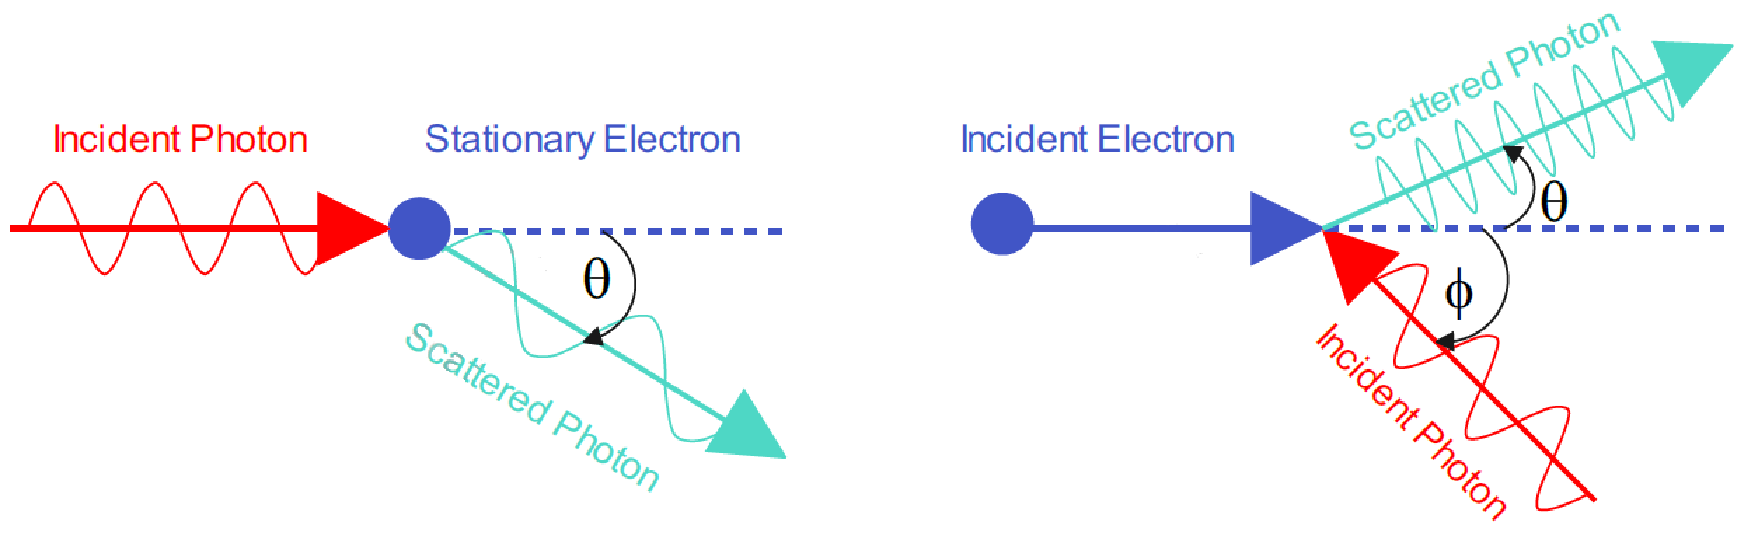
\includegraphics[width=\textwidth]{Figures/Introduction/CS_ICS_diagram_simple_fixed.pdf}
\caption{Left: Compton scattering of a incident photon (red) from a stationary electron where the incident photon is scattered (green) at an angle $\theta$ and decreases in energy, increasing the wavelength, while the stationary electron recoils and gains energy. Right: The inverse Compton scattering interaction where an electron (blue) is interacted with an incident photon (red), typically from a laser, at a crossing angle $\phi$ and scattered to higher energy (frequency) (green) at an scattering angle $\theta$. Energy is transferred from the electron beam to the scattered photon and therefore the electron beam energy is reduced.}
\label{fig:intro_CS_ICS}
\end{figure}

Savedoff \cite{savedoff1959crab} and later Felten and Morrison \cite{felten1963recoil} suggested the use of inverse Compton scattering as a radiation production method, specifically for $\gamma$-rays, which are difficult to obtain due to their inherently short wavelengths (high energies). Though inverse Compton scattering can be conducted with any charged particle, electrons are favoured because their low mass allows for production of high energy radiation and consequently our discussion is limited to electrons. Radiation sources using the principle of inverse Compton scattering can be considered as electron--photon colliders or as `laser undulator' devices. The electron--photon collider model involves a collision between a photon and relativistic electron where the electron recoils and the photon gains energy -- energy is transferred to the incident photon. In the laser undulator description, the large sinusoidally varying electric field of the incident photon pulse causes the electrons to oscillate and therefore emit photons because the electrons are accelerated. The electron bunch in its rest frame radiates as a Hertzian dipole (see Section~\ref{sec:electron_photon_interactions}) but in the laboratory frame the photons are emitted in the direction of the electron motion, into a cone of angle $\theta = 1/\gamma$ due to the Lorentz transformation between the electron rest frame and laboratory frame. The inverse Compton scattering process is illustrated in Fig.~\ref{fig:ICS_frames_diagram}. Both models are equally valid as a consequence of wave--particle duality \cite{de1923waves}, and are used interchangeably to describe particular phenomena. 
\begin{figure}[!h]
\centering
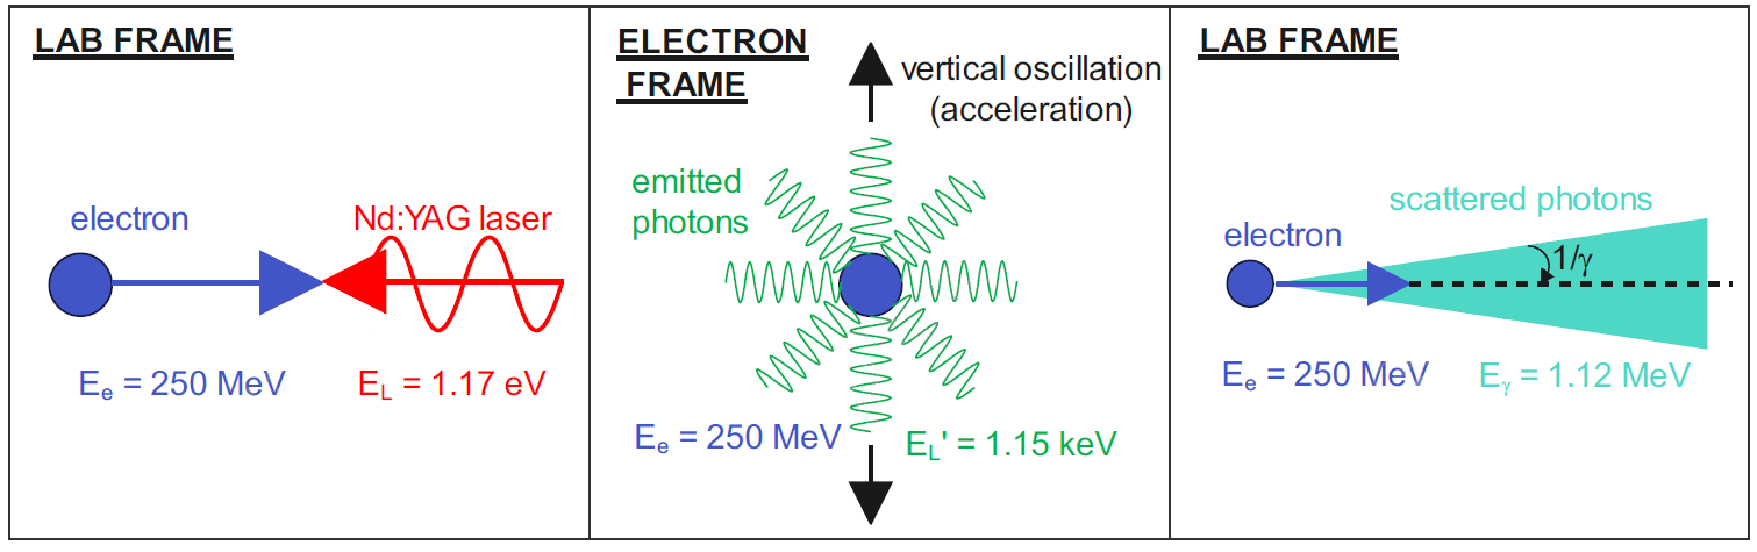
\includegraphics[width=\textwidth]{Figures/Introduction/ICS_diagram_frames_fixed.pdf}
\caption{Diagram of an inverse Compton scattering interaction. Left: An incident photon beam from an Nd:YAG laser ($\lambda = 1064$~\si{\nano\meter}, $E_{L} = 1.17$~\si{\electronvolt}) is incident head-on ($\phi=0$) upon a 250~\si{\mega\electronvolt} electron (blue) (shown in the laboratory frame). Middle: The incident photon is Doppler shifted into the electron rest frame, and hence is boosted to $E_{L}' = 1.15$~\si{\kilo\electronvolt}. As with a Hertizian dipole, the electric field of the incident radiation (incident photons) causes the electron to oscillate vertically and therefore radiate. The photons (green) are emitted isotropically at an identical frequency to the incident radiation, hence photons of $E_{L}' = 1.15$~\si{\kilo\electronvolt} are emitted. Right: The emitted photons are Lorentz transformed to the laboratory frame, and hence are boosted again to an energy of $E_{\gamma} = 1.12$~\si{\mega\electronvolt}. The scattered photons (turquoise) are also emitted into a cone of angle $1/\gamma$ because of this Lorentz transformation, with the scattered photons travelling in the direction of electron propagation.}
\label{fig:ICS_frames_diagram}
\end{figure}

Classically the inverse Compton scattering process can be considered as a double Doppler shift of the incident photon, as shown in Fig.~\ref{fig:ICS_frames_diagram}. Firstly, the incident photon must be Lorentz transformed into the rest frame of the electron via a relativistic Doppler shift
\begin{equation}
f'=\gamma\left(1+\beta\cos\phi\right)f,
\label{eq:Doppler_shift}    
\end{equation}
where $f'$ is the frequency of the incident photon in the electron frame, $f$ is the frequency of the incident photon in the laboratory frame, $\phi$ is the crossing angle between the electron and photon (shown in Fig.~\ref{fig:intro_CS_ICS}), and $\beta = v/c$. If the electron is ultra-relativistic ($\gamma \gg 1$) and the interaction between the electron and photon is head-on ($\phi=0$), the Doppler shift reduces to $f'\approx2\gamma f$. Considering the numerical example in Fig.~\ref{fig:ICS_frames_diagram}, an incident photon from a Nd:YAG laser ($\lambda = 1064$~\si{\nano\meter}, $E_{L} = 1.17$~\si{\electronvolt}) is Doppler boosted to $E_{L}' = 1.15$~\si{\kilo\electronvolt} by a 250~\si{\mega\electronvolt} electron. In the electron rest frame, the incident photon then causes the electron to oscillate and accelerate, emitting photons at the same frequency (energy) as the incident photon which caused the initial acceleration. Then the Lorentz transformation must again be applied to transform the emitted photons from the electron frame back to the laboratory frame via another Doppler shift yielding  
\begin{equation}
f'' \approx 2\gamma^{2}\left(1+\beta\cos\phi\right)f, 
\label{eq:2nd_Doppler_shift}    
\end{equation}
resulting in the frequency, and consequently energy relation for a simplified head-on ($\phi=0$), ultra-relativistic ($\gamma \gg 1$) interaction 
\begin{align}
f'' \approx 4\gamma^{2}f, \nonumber \\
E_{\gamma} \approx 4\gamma^{2}E_{L}
\end{align}
where $E_{\gamma} = hf''$ is the energy of the generated photon and $E_{L} = hf$ is the incident photon energy. In our numerical example this means an initial 1.17~\si{\electronvolt} incident photon can be scattered from a 250~\si{\mega\electronvolt} electron to produce a 1.12~\si{\mega\electronvolt} photon. Therefore, moderate energy particle beams can generate high energy photons from modest incident photon energies. A full quantum derivation of this relationship is shown within Chapter~\ref{Photon_Production_by_Inverse_Compton_Scattering}. 
 
Comparatively, synchrotron radiation production using an LCLS-II undulator (undulator period $\lambda_{u} = 26$~\si{\milli\meter}, magnet flux density $B = 1.01$~\si{\tesla}) \cite{wallen2016status} with a 250~\si{\mega\electronvolt} electron beam yields a photon energy of 15.35~\si{\electronvolt} from the fundamental harmonic -- orders of magnitude below what is available with a `laser undulator'. Therefore, an ICS source allows the generation of sub-angstrom wavelength radiation at modest electron beam energies. However, bremsstrahlung radiation production also allows the production of short wavelengths, for example the Duane--Hunt law (Eq.~\ref{eq:duane_hunt_intro}) shows that a 1~\si{\mega\electronvolt} electron beam can generate photons with energies of up to 1~\si{\mega\electronvolt}, but here the radiation is broadband.

As a radiation production method, a major drawback of the inverse Compton scattering reaction is the low probability of the electron--photon collision, reflected in the total cross section with a typical value close to the Thomson cross section ($\sigma_{T} = 0.665$~\si{\barn}) for electron energies $E_{e} < 1$~\si{\giga\electronvolt} (and decreasing at higher energies). Therefore, generation of large quantities of radiation is challenging. For example, MuCLS -- the current highest flux ICS source demonstrated -- produces up to $1.78\times 10^{10}$~ph/\si{\second} \cite{eggl2016munich} at $E_{\gamma} = 45$~\si{\kilo\electronvolt}, whereas the DIAMOND synchrotron radiation source example in Section~\ref{sec:synchrotron_radiation_intro} showed a flux of $\sim 10^{18}$~ph/\si{\second} and the ARIEL bremsstrahlung source example in Section~\ref{sec:bremsstrahlung} is proposed to generate a flux of $\sim 10^{14}$~ph/\si{\second} at up to $E_{\gamma} = 50$~\si{\mega\electronvolt}. However, the ICS interaction is beneficial over bremsstrahlung and synchrotron radiation because, as demonstrated in Section~\ref{sec:electron_photon_interactions}, there is an energy--angle correspondence, since photons of a particular energy $E_{\gamma}$ are scattered into a particular scattering angle $\theta$, which allows certain energy photons to be selected by a simple collimator and a narrow bandwidth can be obtained. A similar energy--angle correspondence does not exist in synchrotron or bremsstrahlung radiation production, therefore this is a unique feature of inverse Compton scattering. Use of inverse Compton scattering as a radiation production method is further explored in Chapter~\ref{Photon_Production_by_Inverse_Compton_Scattering}. 

\section{Thesis Layout and Scope}
\label{sec:thesis_layout_scope}

The thesis is concerned with the investigation of high-energy radiation production via the interaction of ultra-relativistic electron beams with laser pulses -- known as inverse Compton scattering -- where the electron bunch is generated using an energy recovery linac. Therefore, the thesis has three main foci: 
\begin{enumerate}
    \item{Possible designs of ERL driven ICS sources, with comparison of ERL drivers to other accelerator types.}
    \item{The optimum configuration of the electron beam for operation of ICS sources as high flux, narrow bandwidth light sources most favoured by experimentalists.}
    \item{Identification of suitable applications for an ERL driven ICS source, with reference to ERL driven ICS design parameters, and comparison against other accelerator light sources.}
\end{enumerate}

Consequently, the thesis is structured as follows. Firstly,  Chapter~\ref{Energy_Recovery_Linac_Design} presents an overview of the beam dynamics considerations for design of an ERL based ICS source, then the theory relevant to characterisation and design of an inverse Compton scattering source is presented in Chapter~\ref{Photon_Production_by_Inverse_Compton_Scattering}. Developed methods for optimisation and characterisation of ICS sources are explained and demonstrated in Chapter~\ref{Optimisation_and_Characterisation_of_Inverse_Compton Scattering_Spectra}. Improvements in the characterisation of an ICS source are made via the derivation of an analytical calculation for the flux of an ICS source post-collimation and creation of a semi-analytical spectrum code named \textsc{ICARUS}. A series of optimisations of transverse electron bunch parameters for high flux, narrow bandwidth radiation are produced. The methods developed in Chapter~\ref{Optimisation_and_Characterisation_of_Inverse_Compton Scattering_Spectra} are applied to designs of ERL driven ICS sources in the rest of the thesis. In Chapter~\ref{CBETA_Inverse_Compton_Scattering_Source_Design} an x-ray ERL driven source design based upon CBETA -- the worlds first multi-turn SRF ERL -- is produced, characterised and compared with other competing x-ray sources. Potential applications of such a source are explained. Understanding the application of ICS sources to x-ray production then led to design of a $\gamma$-ray ICS source utilising the conceptual DIANA ERL in Chapter~\ref{DIANA_Inverse_Compton_Source_Design}. The DIANA $\gamma$-ray ICS source design is optimised, characterised and compared to bremsstrahlung $\gamma$-ray production with investigation of several applications. Finally, in Chapter~\ref{Conclusion} the main findings throughout the thesis are re-iterated and future work relevant to ERL driven ICS sources is discussed.       

\end{document}